%\subsection{Experiment 2.2: Initial Entropy Experiments}
%
%\paragraph{Overview}

%\paragraph{Andrews notes} You've got a lot of files, and results, but give some 
%careful thought as to how you might perform a statistical test to compare the 
%results obtained and see if there is a difference. 
%
%For example, the most obvious 
%one would be to calculate the statistics, eg say at least mean and variance of the 
%entropy across all the speakers and then see if you can detect any statistically 
%significant differences when you consider male/female. This in itself would be of 
%interest, regardless of the outcome. 
%
%
%
%
%See if I can build a model of general mean of the entropy values and of the variance. \\
%Find two good output files that have very different speech patterns and see if 
%this can be shown to dip or raise entropy in the anomaly plots \\
%
%What are the numbers? Was there only one entorpy value??? Or is that an average? So would this be the parameter for a gaussian of these entropy models?
%
%Would we say thay anything outside of 60\% of 95\% is an outlier then? Maybe we can take the average of all the averages and the average of all the variances and build an classification model with that?  
%
%Where does the ranked probability graph come into it then? Where I'm showing the 



\clearpage
\section{Experiment 2.1 - Entropy Analysis of Unaugmented Audio}
%\subsubsection{Experiment Overview}
%
%File: aaj-2019-05-09\\
%Binary Pause Total Length(Audio file length): 31777 \\
%Total Binary Pauses (Non-utterance?): 25444\\
%Total Binary Sounding: 6333\\
%Number of Pauses: 3560\\
%Pause Proportion: 0.801\%\\
%Average Pause Length: 7.14\\
%Symbol Set: [(2705, 'A'), (855, 'B')] \\
%Window size: 100 \\
%Window overlap: 0, 40, 80 \\
%Maximum Entropy: 1 \\
%Pause Profile Mean: 7.145\\
%Pause Profile Variance: 65.300\\

\subsection{Experiment 2.1.1 - Window Overlap}
This experiment looked at the change window overlap had on the entropy profile. The figure shows three different window overlaps of 0, 40, 80, window size of 100 stays consistent throughout used on file aaj-2019-05-09 with SM[10].


\begin{table}[htp]
	\begin{center}
	\begin{tabular}{|c|c|c|}
		\hline
		\multicolumn{3}{|c|}{Entropy Profile Data using Symbol Model [10]} \\%
		\hline
		{\small Overlap} & {\small Mean} & {\footnotesize Variance} \\
		\hline \hline
		0 & 0.781 & 0.010 \\
		40 & 0.781 & 0.012 \\
		80 & 0.783 & 0.010 \\
		\hline   
	\end{tabular}
	\label{tab:2}
	\caption{Analysing data collected from all the female only pause files on different metrics, what are the numbers?}
	\end{center}
\end{table}%
%Entropy Profile Mean - Window overlap \\
%Entropy Profile Variance - Window overlap 0: \\
%Entropy Profile Mean - Window overlap 40: \\
%Entropy Profile Variance - Window overlap 40: \\
%Entropy Profile Mean - Window overlap 80: 3\\
%Entropy Profile Variance - Window overlap 40: \\
\begin{figure}[b]
\begin{center}
	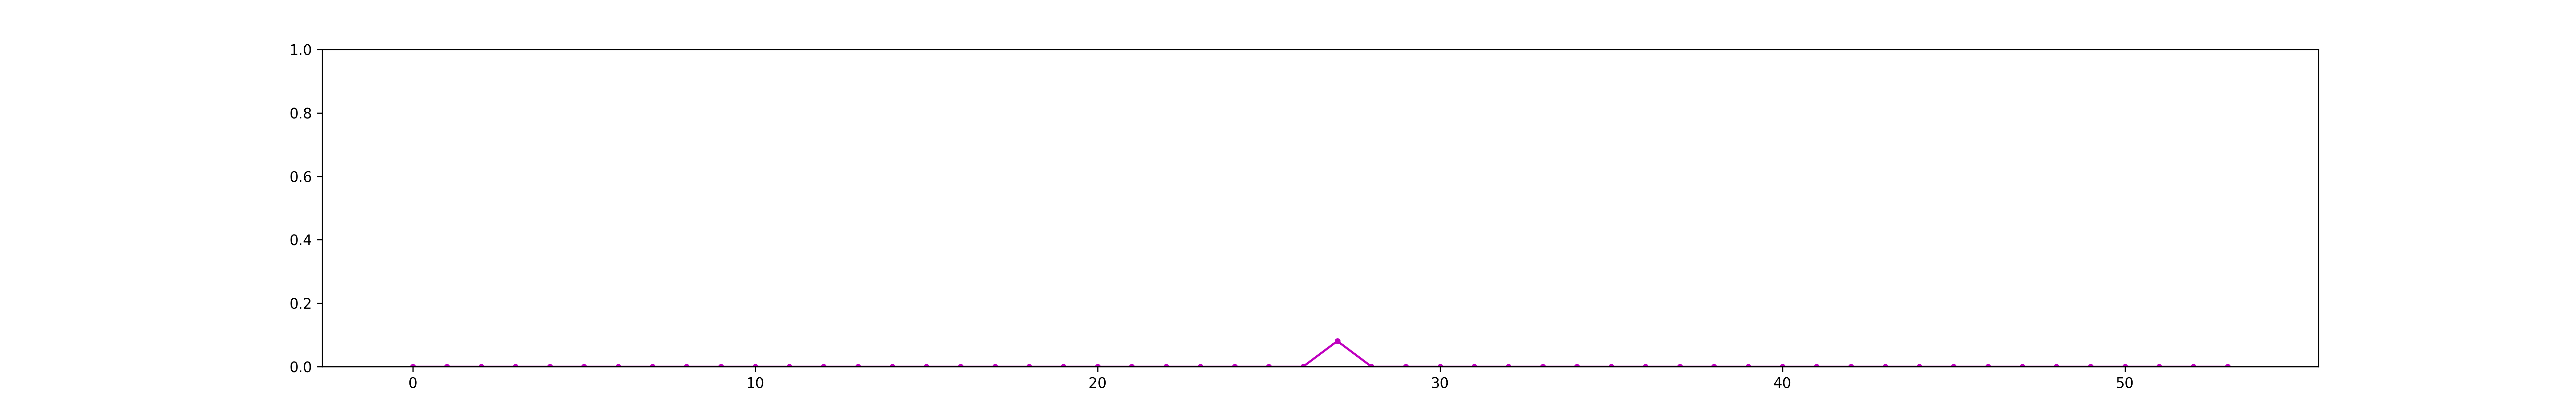
\includegraphics[scale=0.15]{src/main-matter/results/experiment-age/entropy/[10]/Overlap(0)}
	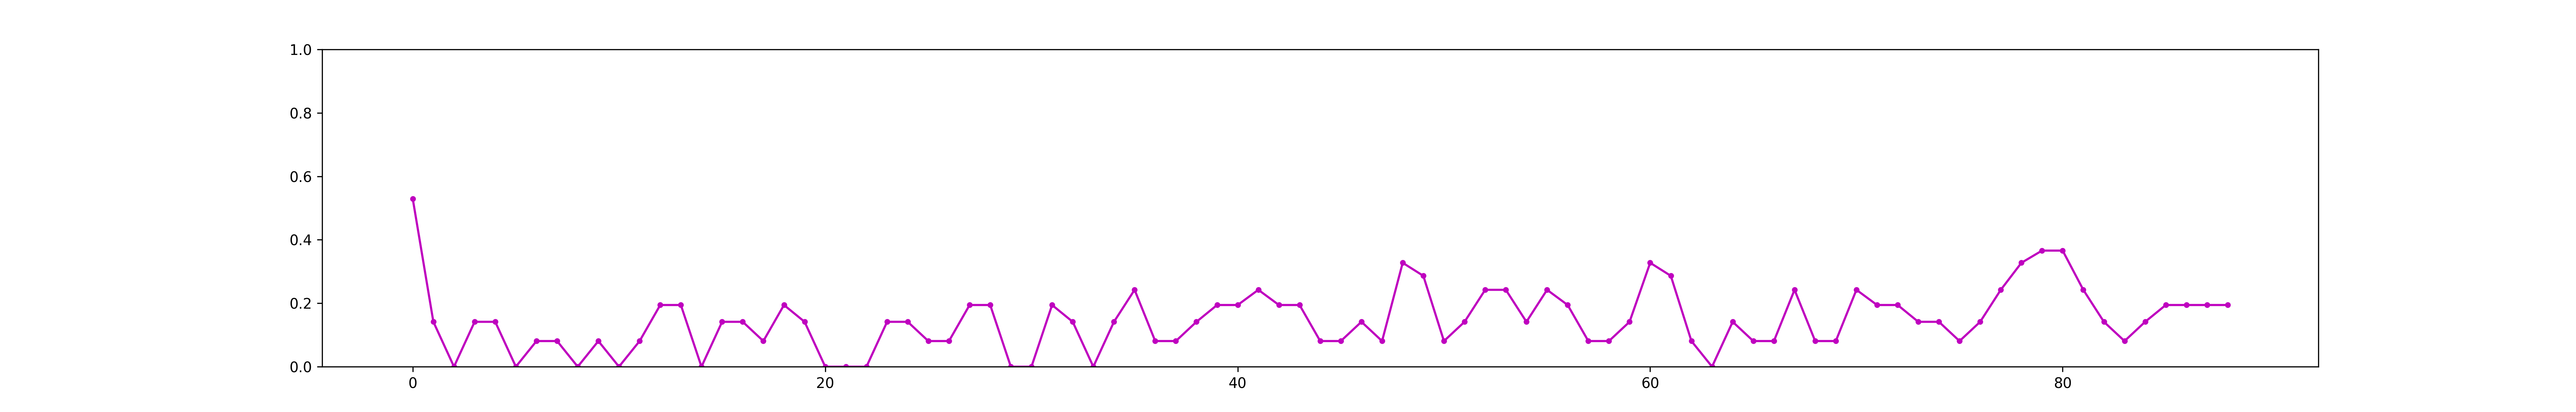
\includegraphics[scale=0.15]{src/main-matter/results/experiment-age/entropy/[10]/Overlap(40)}
	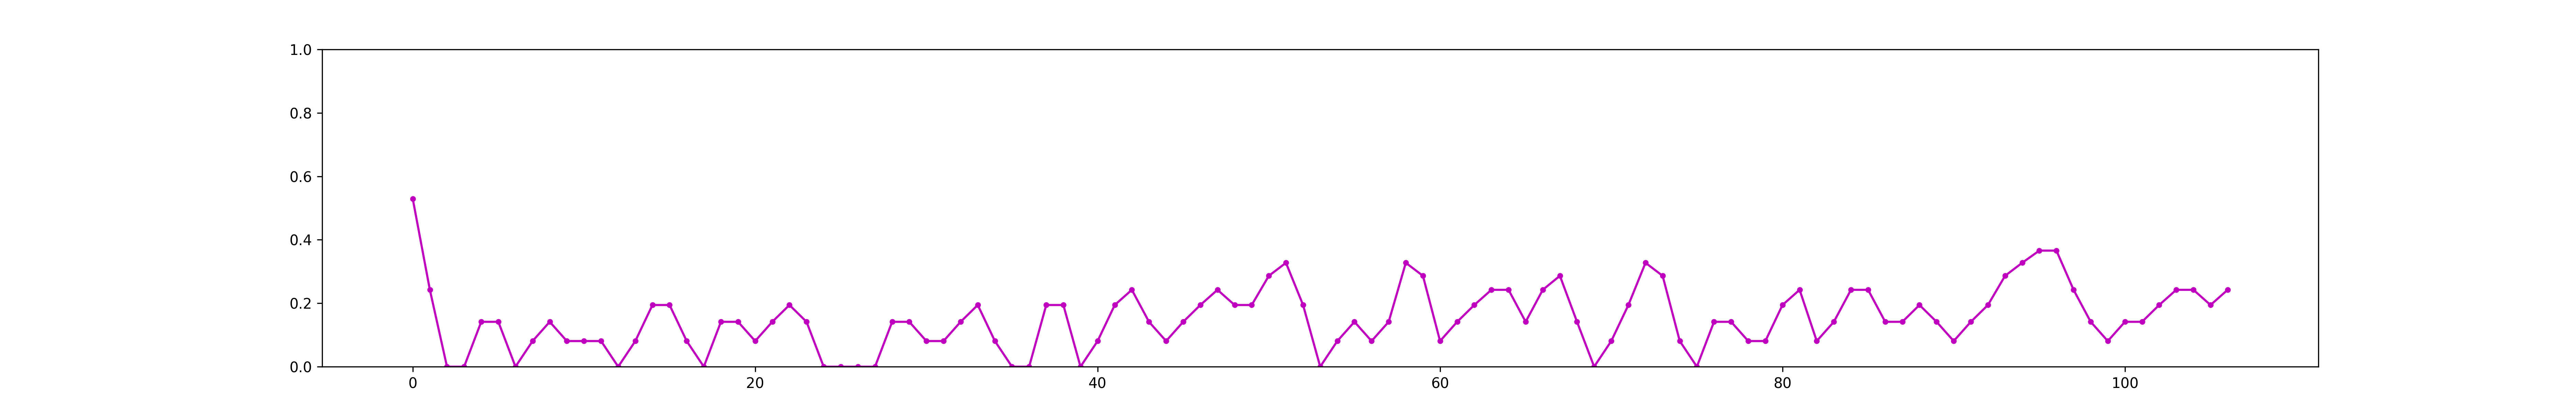
\includegraphics[scale=0.15]{src/main-matter/results/experiment-age/entropy/[10]/Overlap(50)}
	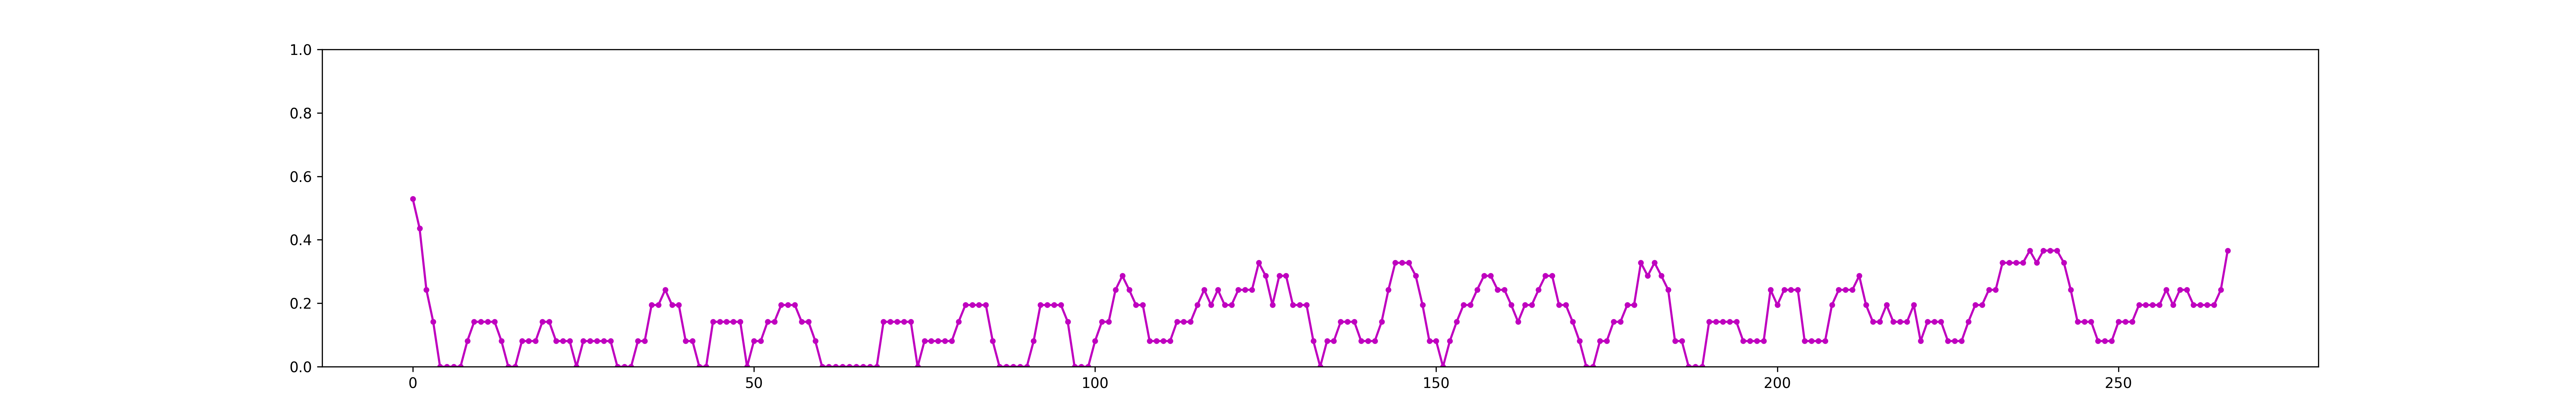
\includegraphics[scale=0.15]{src/main-matter/results/experiment-age/entropy/[10]/Overlap(80)}
	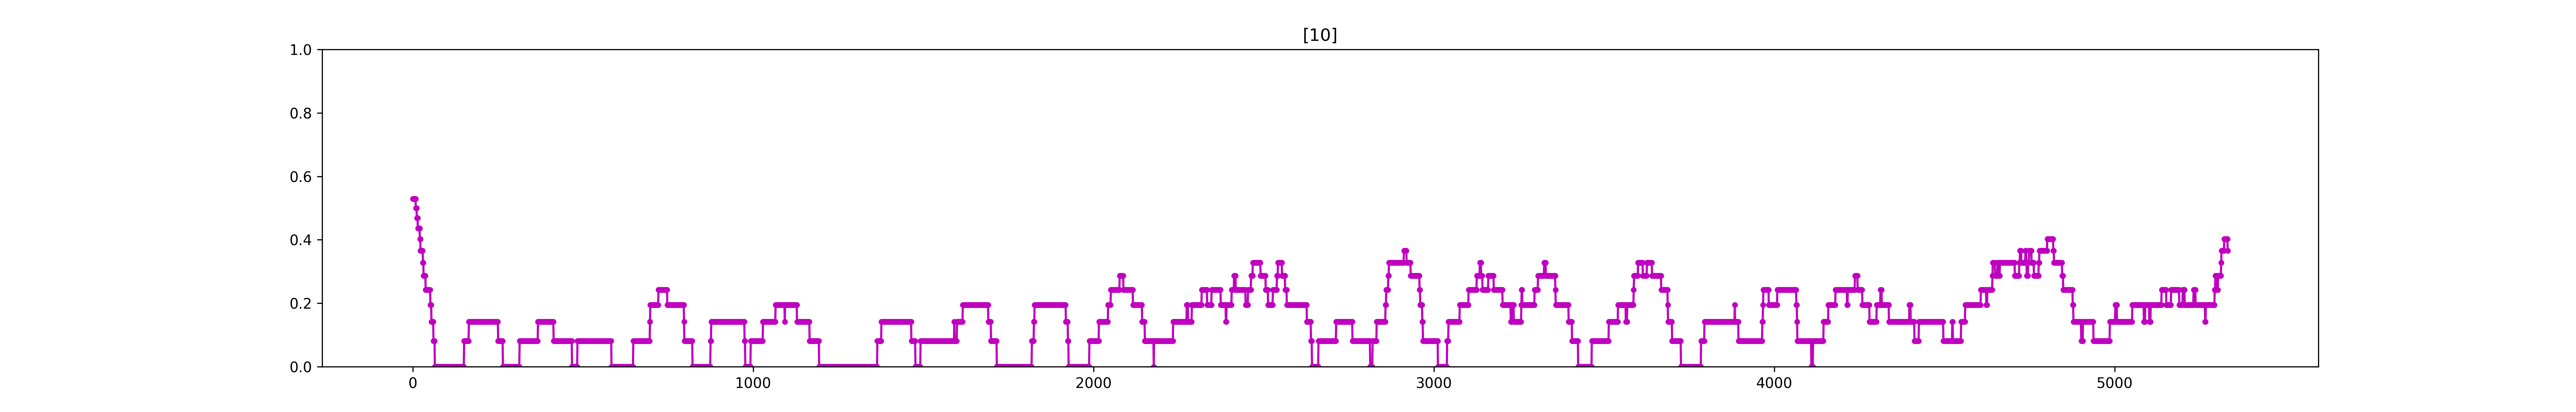
\includegraphics[scale=0.15]{src/main-matter/results/experiment-age/entropy/[10]/Overlap(99)}
\caption{Experiment 2.1.1: Investigating the effects overlap has on the entropy profile structure for file aaj-2019-04-26 using SM[10]. Overlap values of 0, 40, 50, 80, 99 from top to bottom respectively. Window size of 100 was used throughout.}
\label{default}
\end{center}
\end{figure}






\subsection{Experiment 2.1.2 - Window Size}
This experiment looked at the change window size had on the entropy profile. The figure shows three different sizes of 50, 100 and 250. Window overlap stays consistent throughout as window\_overlap = window\_size - 1.

\begin{figure}[h]
\begin{center}
	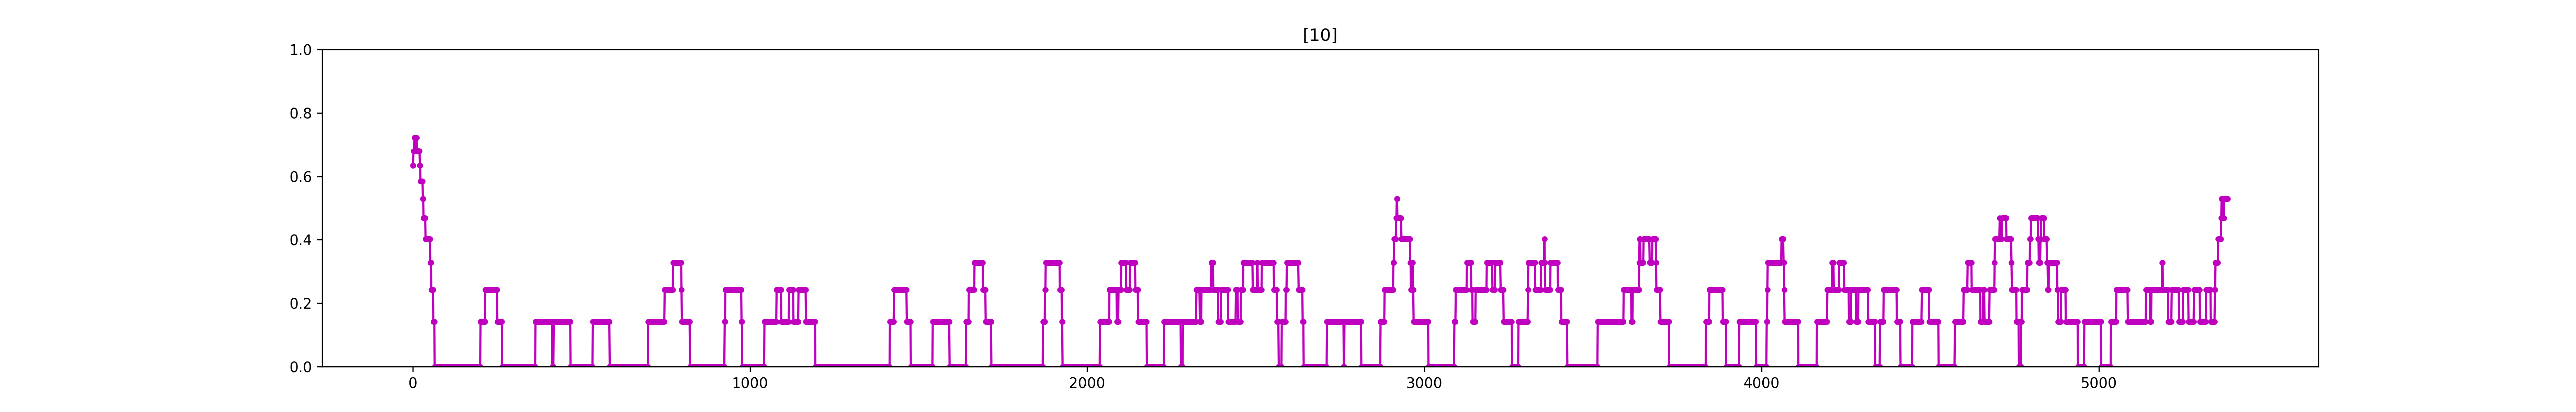
\includegraphics[scale=0.15]{src/main-matter/results/experiment-age/entropy/[10]/WindowSize(50)}
	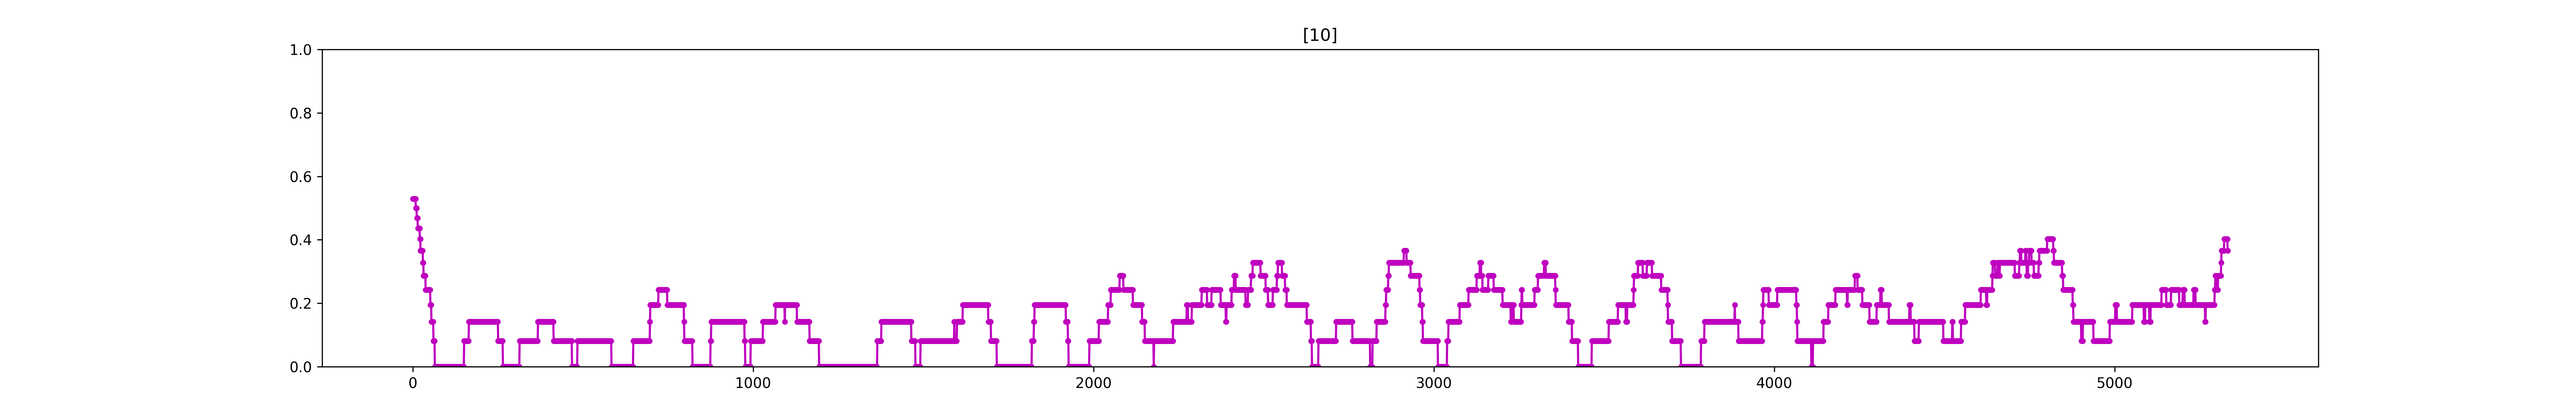
\includegraphics[scale=0.15]{src/main-matter/results/experiment-age/entropy/[10]/WindowSize(100)}
	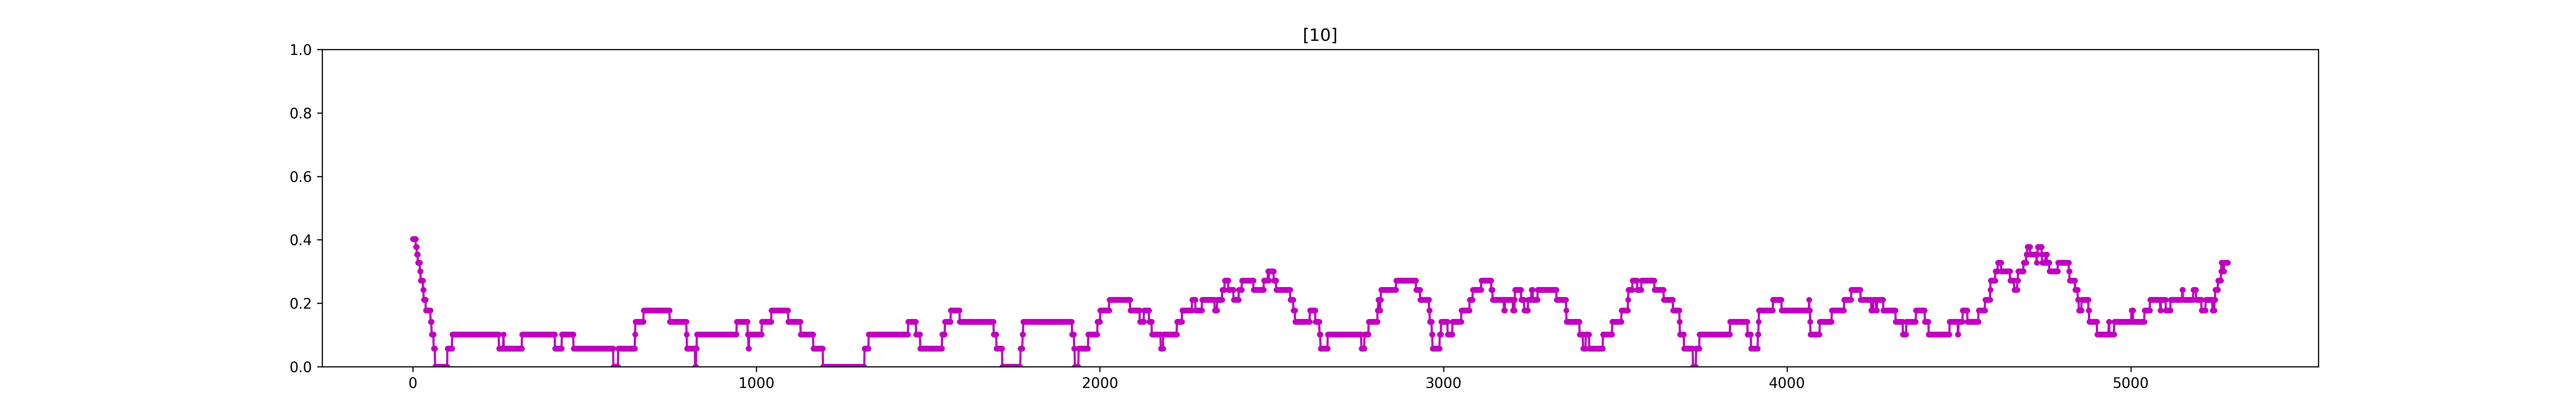
\includegraphics[scale=0.15]{src/main-matter/results/experiment-age/entropy/[10]/WindowSize(150)}
	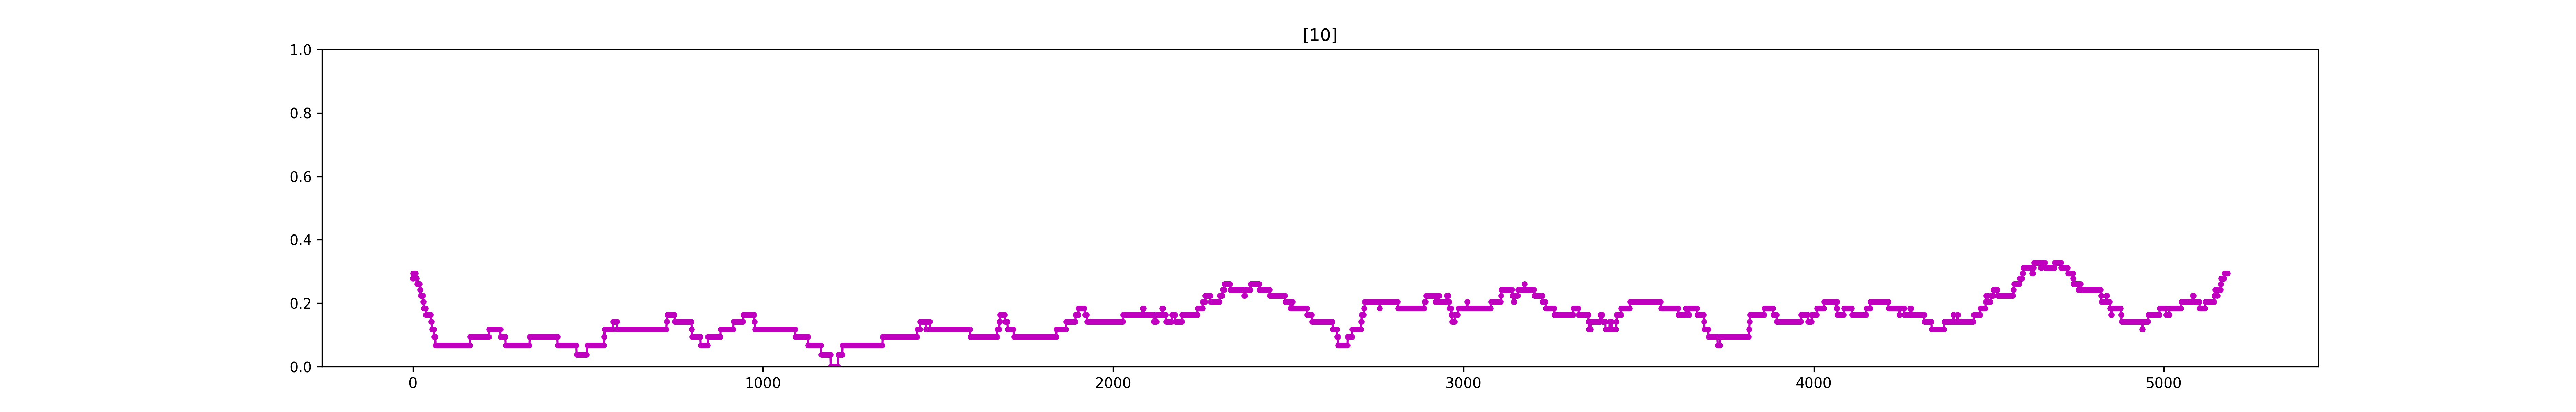
\includegraphics[scale=0.15]{src/main-matter/results/experiment-age/entropy/[10]/WindowSize(250)}
	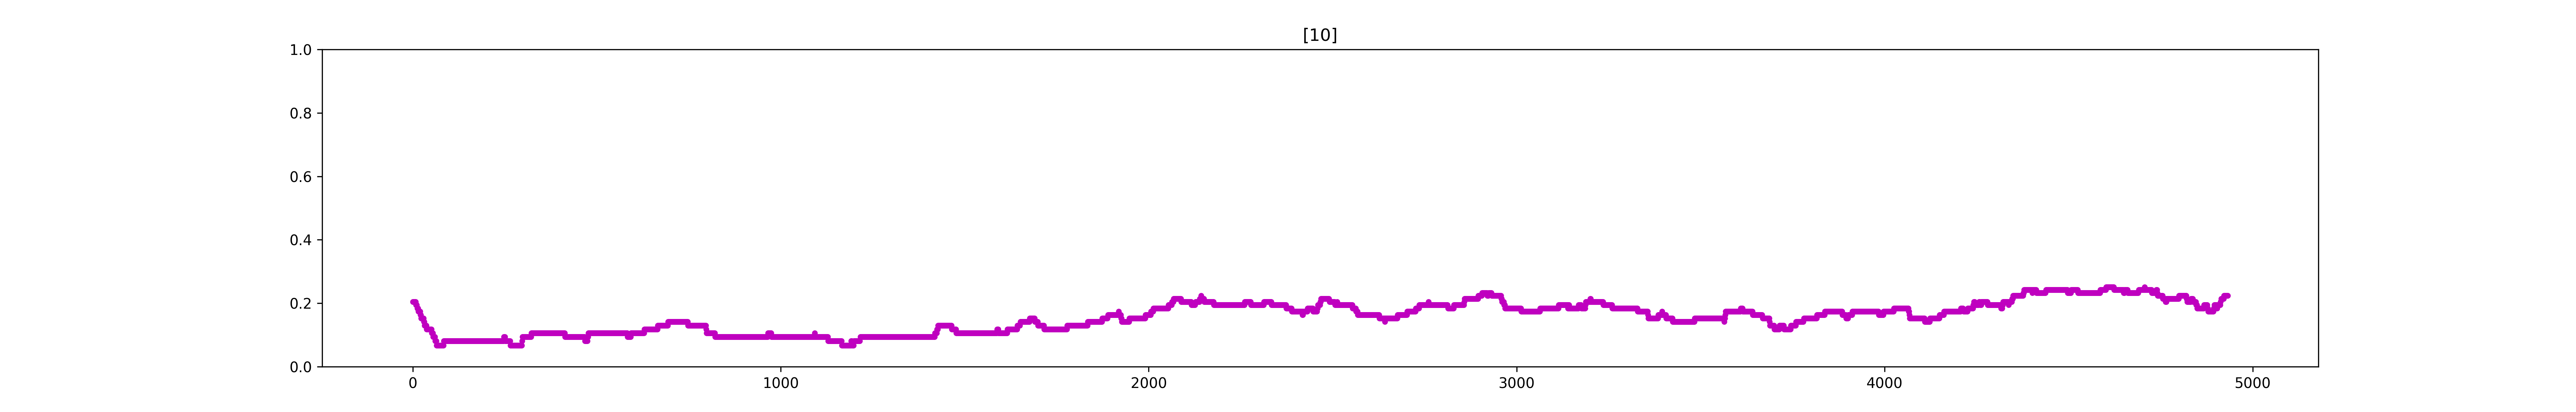
\includegraphics[scale=0.15]{src/main-matter/results/experiment-age/entropy/[10]/WindowSize(500)}
\caption{Experiment 2.2.2:  Investigating the effects window size has on the entropy profile structure for file aaj-2019-04-26 using SM[10]. Window size of 50, 100, 150, 250, 500 from top to bottom respectively}
\label{default}
\end{center}
\end{figure}




%\clearpage


\subsection{Experiment 2.1.3 - Entropy Profiles of SA1}
\subsubsection{Experiment 2.1.3.1 - SM[3]}
    \begin{figure}[h]
    \begin{center}
    	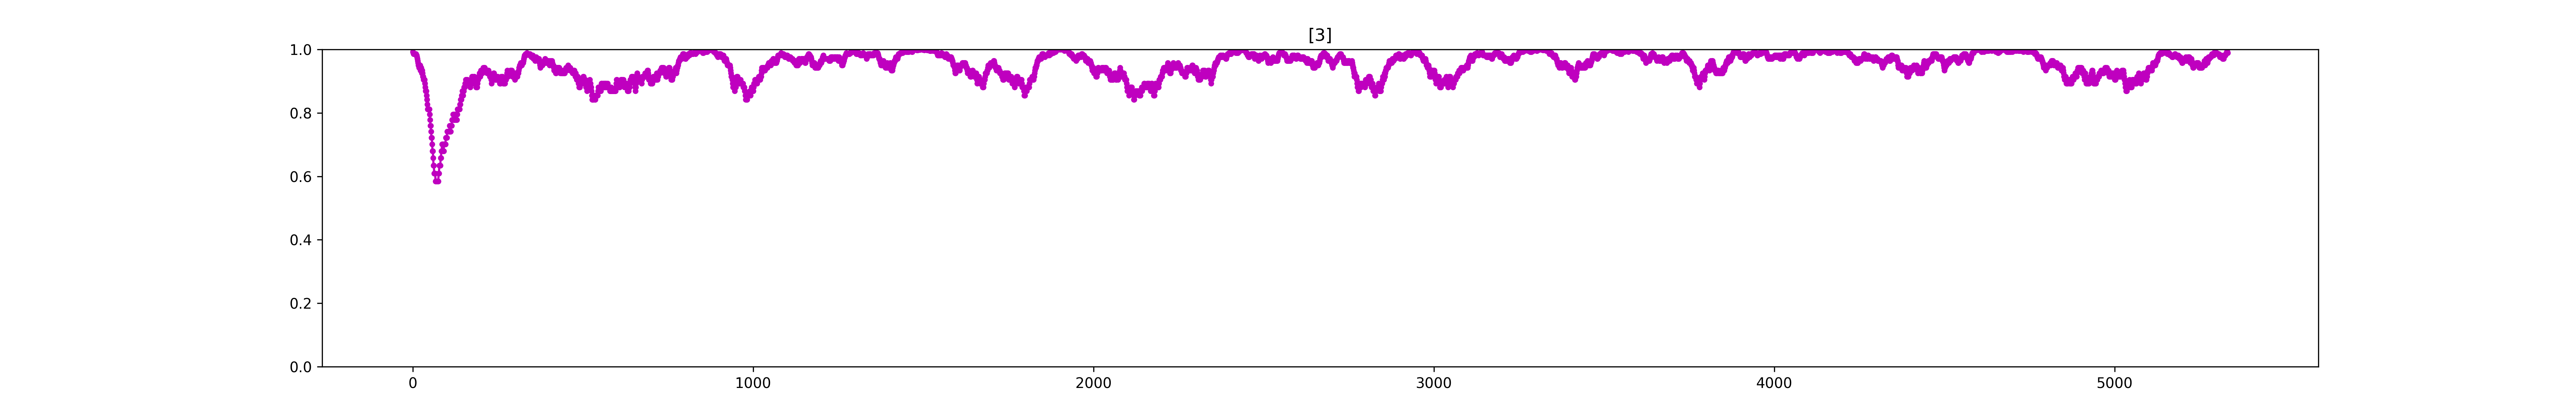
\includegraphics[scale=0.2]{src/main-matter/results/experiment-age/entropy/window100/[3]}
    \caption{Investigating the entropy profile structure for file aaj-2019-04-26 using SA1 - SM[3]}
    \label{default}
    \end{center}
    \end{figure}

\clearpage

\subsection{Experiment 2.1.4 - Entropy Profiles of Increasing Bin Width}
\subsubsection{Experiment 2.1.4.1 - SM[10]}
 Ranked Probability: [(5294, 'A'), (138, 'B')]
    \begin{figure}[h]
    \begin{center}
    	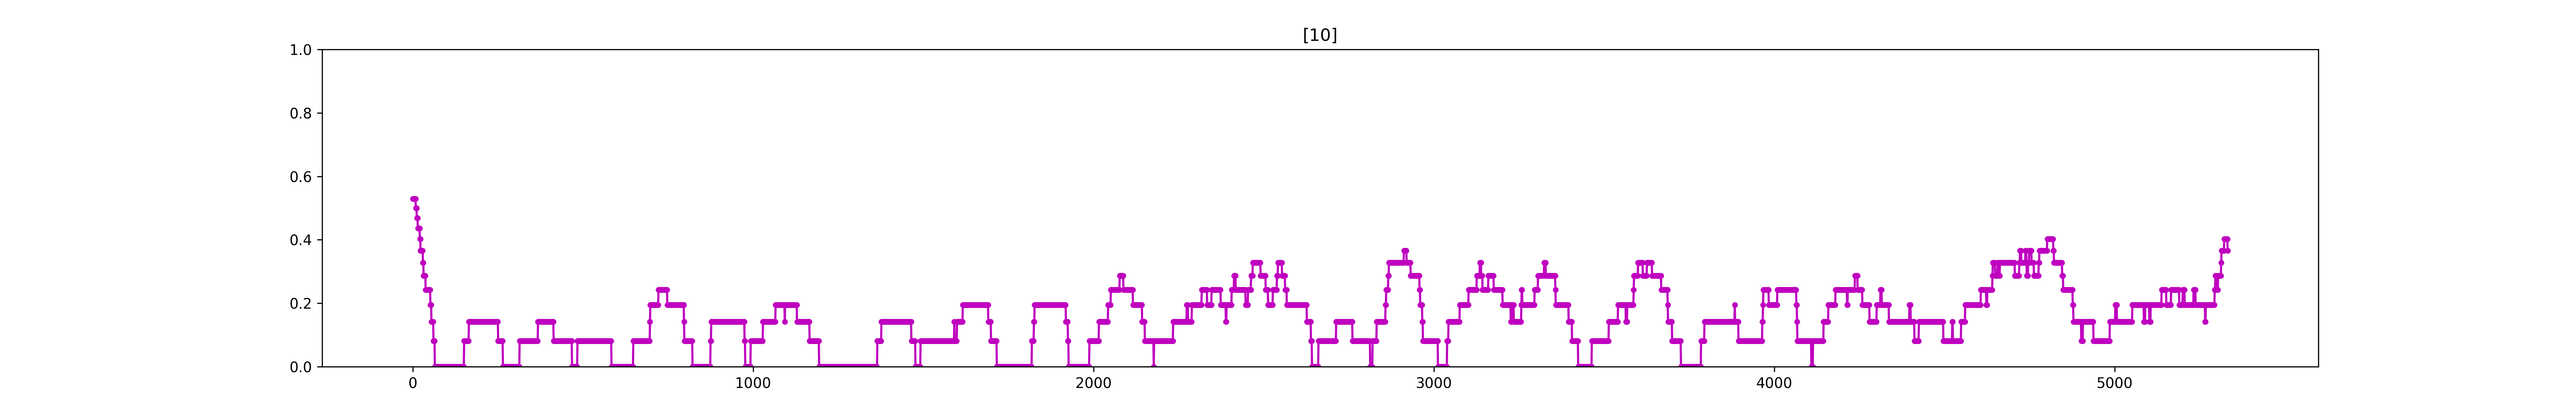
\includegraphics[scale=0.2]{src/main-matter/results/experiment-age/entropy/window100/[10]}
    \caption{Investigating the entropy profile structure for file aaj-2019-04-26 by increasing the bin width of SA1 - SM[10]}
    \label{default}
    \end{center}
    \end{figure}

\subsubsection{Experiment 2.1.4.2 - SM[20]}
    \begin{figure}[h]
    \begin{center}
    	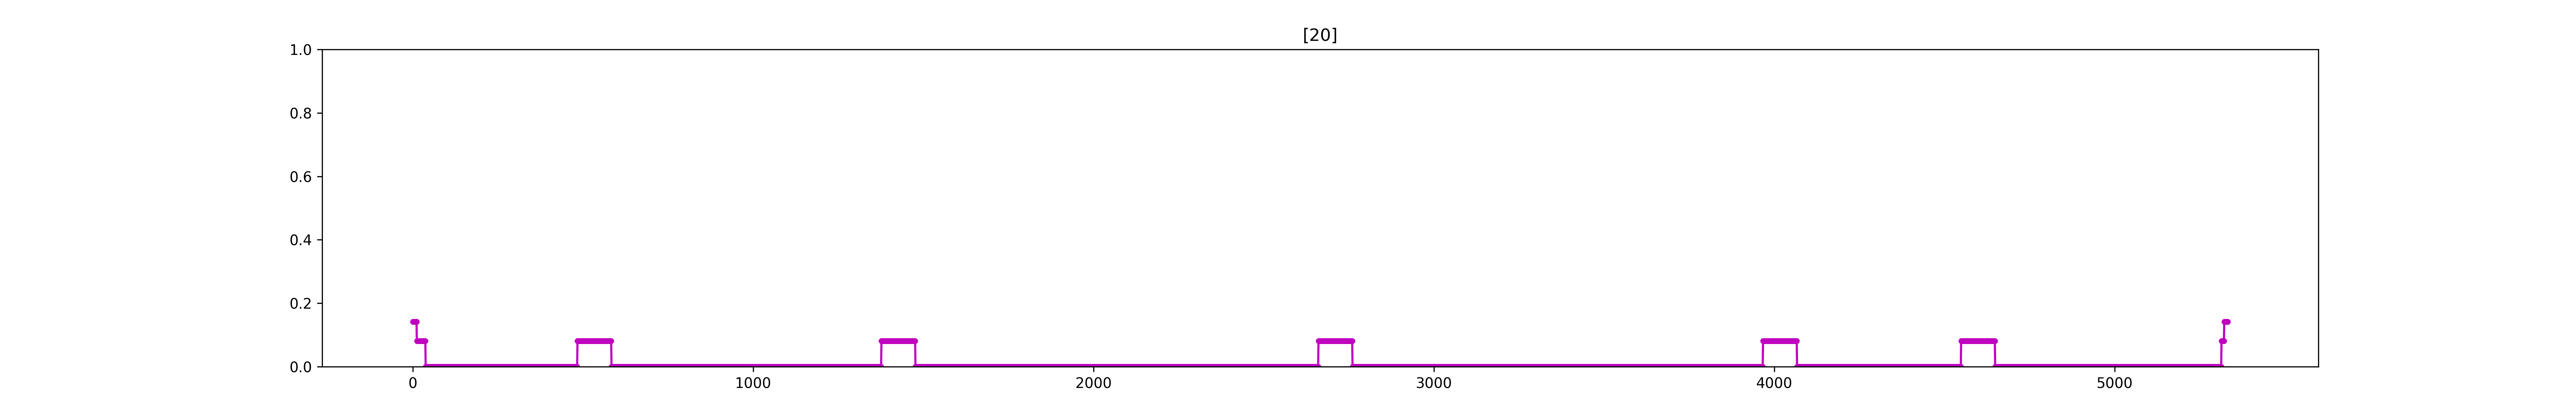
\includegraphics[scale=0.2]{src/main-matter/results/experiment-age/entropy/window100/[20]}
    \caption{Investigating the entropy profile structure for file aaj-2019-04-26 by increasing the bin width of SA1 - SM[20]}
    \label{default}
    \end{center}
    \end{figure}

%\subsection{Experiment 2.2.3 - Outlier Significance - [35]}

%(i.e. making the occurrence of the second symbol as small as possible to make its occurrence rare, thus increasing outlier significance). 
%
%Symbol Model: [35]\\ 
%Symbolisation approach: SA0.1\\ 
%File: aaj-2019-03-15 (from experiment 1) \\ 
%Window size: 100 \\
%Overlap: 0\\
%Ranked Probability: [(3509, 'A'), (51, 'B')] \\


%\subsubsection{Experiment 2.1.3.4 - SM[35]}
%\begin{figure}[h!]
%\begin{center}
%	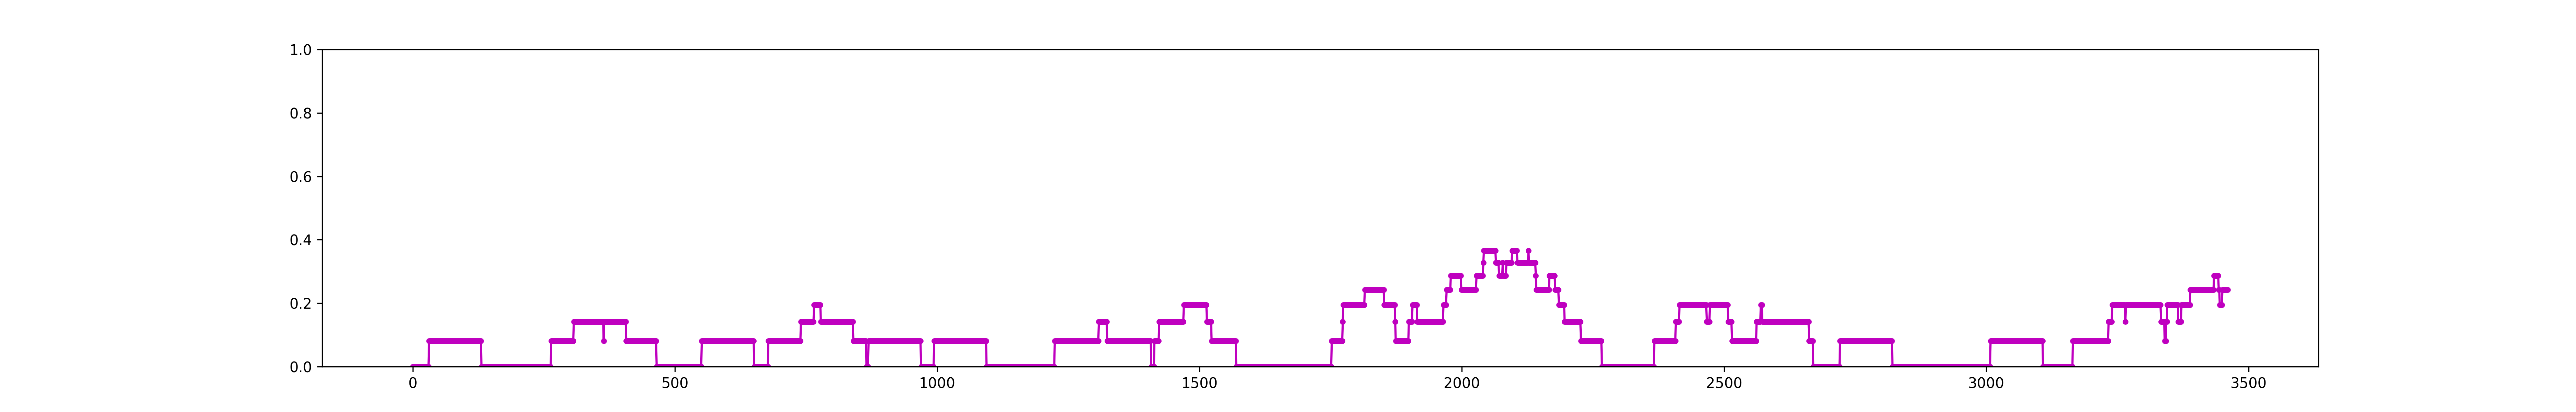
\includegraphics[scale=0.2]{src/main-matter/results/experiment-age/entropy/[35]/Overlap(99)}
%\caption{Experiment Outlier Significance for Overlap 0, 50, 99 respectively}
%\label{default}
%\end{center}
%\end{figure}


%
%
%\subsubsection{Experiment 3 - [50]}
%Using the symbol model [50] produced a single anomaly at the end. Showing that only one anomaly is required for it to be displayed.
%
%\subsubsection{Experiment 4 - [20,50]}
%Using the symbol model [20, 50] produced identical results to exp 1
%
%\subsubsection{Experiment 5 - [10,20,50]}


\subsection{Experiment 2.1.5 - Entropy Profile of SA2}
    \begin{figure}[h]
    \begin{center}
    	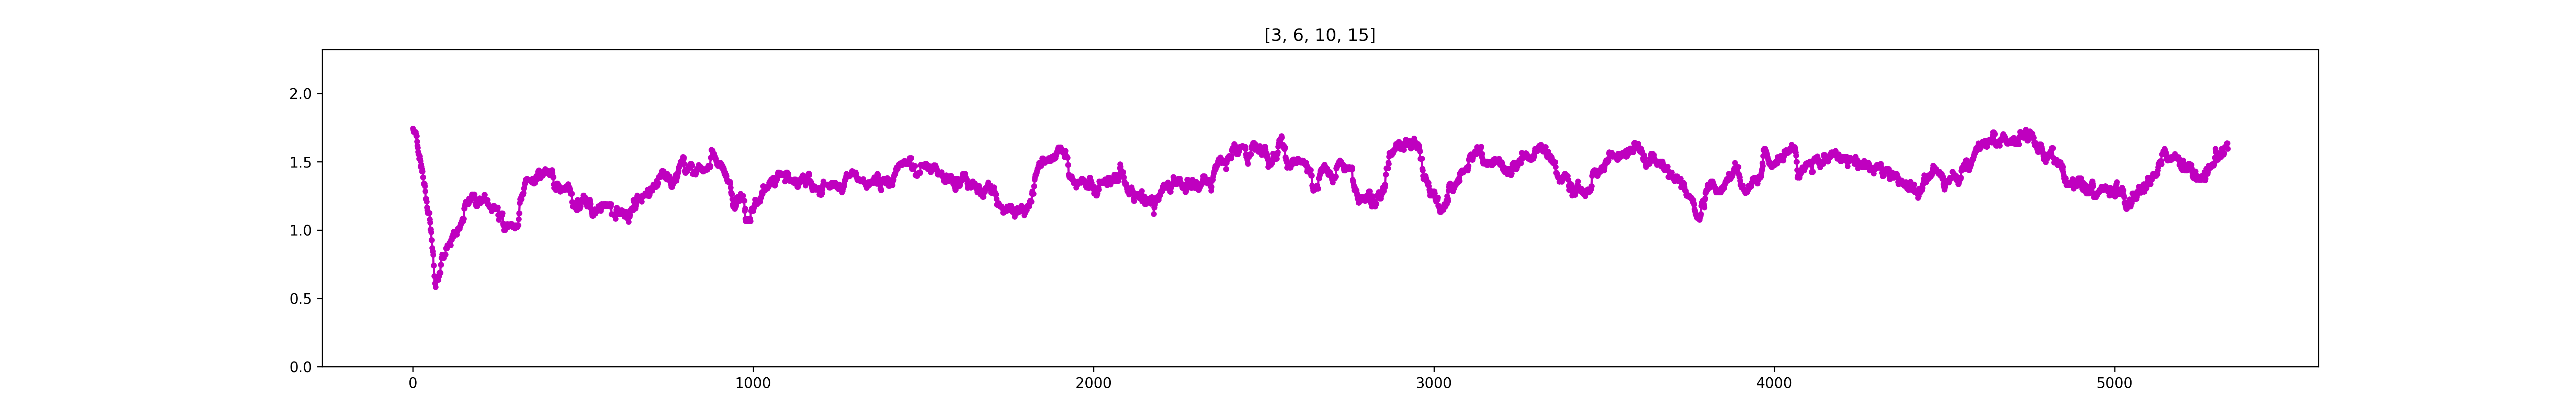
\includegraphics[scale=0.2]{src/main-matter/results/experiment-age/entropy/window100/[3,6,10,15]}
    \caption{nvestigating the entropy profile structure for file aaj-2019-04-26 by using SA2 - SM[3,6,10,15]}
    \label{default}
    \end{center}
    \end{figure}
%\paragraph{Mean}
%Mean was --
%
%\paragraph{Range}
%Range was roughly the same for both \\
%
%\paragraph{Variance}
%ABC was much less consistent, varying between the range values constantly meaning frequent change in information delivery. \\

%\begin{table}[htp]
%	\begin{center}
%	\begin{tabular}{|c|c|c|c|}
%		\hline
%		\multicolumn{4}{|c|}{JJJ Entropy Data using S1 Symbol Model} \\%
%		\hline
%		{\small Data} & {\small Standard Mean} & {\footnotesize Geometric Mean????} & {\footnotesize Variance} \\
%		\hline \hline
%		4889 & 4.146 & - & 0.0008120 \\
%		\hline   
%	\end{tabular}
%	\label{tab:2}
%	\caption{Analysing data collected from all the female only pause files on different metrics, what are the numbers?}
%	\end{center}
%\end{table}%



\clearpage


\section{Augmented Audio Experiments}
%\subsection{Single 30s Pause Insertion}
%aaj-2019-04-24?
%Using the audio file aaj-2019-03-15 a single 30s long pause was inserted into the audio at the 50 minute mark to see how the symbol models produced do in showing anomalies.   
%\subsubsection{Exp5 - [10]}
% Symbol model ... showed the 
% 
% \paragraph{Mean}
%Mean was --
%
%\paragraph{Range}
%Range was roughly the same for both \\
%
%\paragraph{Variance}
%ABC was much less consistent, varying between the range values constantly meaning frequent change in information delivery. \\
%
% \subsubsection{Exp6 - [20]}
% 
%  \subsubsection{Exp7 - [2, 3, 4, 5, 6, 7, 8, 9, 10]}

 \begin{table}[htp]
	\scriptsize
	\begin{center}
	\begin{tabular}
		{ 
			|p{1.5cm}| |p
			{1.5cm}|p
			{.8cm}|p
			{.8cm}|p
			{.8cm}|p
			{.8cm}|
		}
		\hline
		\multicolumn{6}{|c|}{ABC - Radio - Program: Conversations} \\%
		\hline
			{\footnotesize Audio File} & 
			{\scriptsize Entropy Variance} & 
			{\scriptsize Mode} &
			{\scriptsize Mean} &
			{\scriptsize Median} & 
			{\scriptsize Range} \\
		\hline
		\hline

		%\cellcolor[HTML]{A2A1A2} 
		aaj-2019-03-15 & 41 - 47 & 44 & - & - & 6 \\
		\hline 
		aaj-2019-03-21 & 40 - 48 & 44 & - & - & 8 \\
		\hline 
		aaj-2019-03-27 & 38 - 42 & 40 & - & - & 4 \\
		\hline
		aaj-2019-04-11 & 37 - 43 & 40 & - & - & 6 \\
		\hline
		aaj-2019-04-24 & 37 - 43 & 40 & - & - & 6\\
		\hline
		aaj-2019-04-26 & 41 - 48 & 44 & - & - & 7 \\
		\hline
		aaj-2019-04-29 & 38 - 46 & 42 & - & - & 8 \\
		\hline
		aaj-2019-04-30 & - & - & - & - & - \\
		\hline
		aaj-2019-05-17 & - & - & - & - & - \\
		\hline
		aaj-2019-05-08 & - & - & - & - & - \\
		\hline
		aaj-2019-05-09 & - & - & - & - & - \\
		\hline
		\hline 
		Average & - & - & - & - & 6.43 \\
		\hline
		\hline

	\end{tabular}
	\label{tab:1}
	\caption{Pause usage of abc conversations audio files - preliminary statistical pause analysis 
	pertaining to middle aged participants with the results of SM.1 on each audio file with the total pauses
	 for that file and the pauses counted for each symbol} \\
	\end{center}
\end{table}


 \begin{table}[htp]
	\scriptsize
	\begin{center}
	\begin{tabular}
		{ 
			|p{1.5cm}| |p
			{1.5cm}|p
			{.8cm}|p
			{.8cm}|p
			{.8cm}|p
			{.8cm}|
		}
		\hline
		\multicolumn{6}{|c|}{ABC - Radio - Program: Mornings} \\%
		\hline
			{\footnotesize Audio File} & 
			{\scriptsize Entropy Variance} & 
			{\scriptsize Mode} &
			{\scriptsize Mean} &
			{\scriptsize Median} & 
			{\scriptsize Range} \\
		\hline
		\hline

		%\cellcolor[HTML]{A2A1A2} 
		- & 38 - 42 & 40 & - & - & 4 \\
		\hline 
		-- & 37 - 41 & 39 & - & - & 4 \\
		\hline 
		--- & 37.5 - 41.5 & 39.5 & - & - & 4 \\
		\hline
		-- & 40 - 44 & 42 & - & - & 4 \\
		\hline
		-- & 37 - 42 & 39 & - & - & 5\\
		\hline
		--- & 38.5 - 41.5 & 40 & - & - & 3 \\
		\hline
		-- & 38 - 42 & 40 & - & - & 4 \\
		\hline
		---- & - & - & - & - & - \\
		\hline
		-- & - & - & - & - & - \\
		\hline
		-- & - & - & - & - & - \\
		\hline
		-- & - & - & - & - & - \\
		\hline
		\hline 
		Average & - & - & - & - & 4 \\
		\hline
		\hline

	\end{tabular}
	\label{tab:1}
	\caption{Pause usage of abc conversations audio files - preliminary statistical pause analysis 
	pertaining to middle aged participants with the results of SM.1 on each audio file with the total pauses
	 for that file and the pauses counted for each symbol} \\
	\end{center}
\end{table}




So what does high entropy mean, greater distributed use of the symbols? 

What does high variance mean then? Inconsistent use of pauses. Maybe it was the style of conversation? 

How is it higher variance? Are they hitting higher peaks? Lower troughs? 

What does it tell us about the groups? Maybe the longer length of conv allowed for different use of pauses (relaxed? does that account for the variance?)

This shows the variance tends to be greater for --- conversations, indicating the information theyre giving tends to move from high information to low more frequently whereas -- people tend to stick to a common entropy value more often.

Not only were the outlier points greater for conversations, but I think they tended to fluctuate more often between those points.



%
%\paragraph{Mean}
%Mean was --
%
%\paragraph{Range}
%Range was roughly the same for both \\
%
%\paragraph{Variance}
%ABC was much less consistent, varying between the range values constantly meaning frequent change in information delivery. \\
%
%\subsection{Write up about all the things from the poster I did}
%
%\subsubsection{Exp x - [3,6,10,15]}
%This is the model that was used in the presentation. This was good firstly because it showed the data wasn't uniform or completely predictable, but rather showed levels of predictability, meaning inferences could be made. Secondly it showed the pause distribution to be really similar to the zml curve, such that modelling it with the fast entropy system should be very simple given the already existing similar results from [andrews paper].  
%
%\paragraph{Mean}
%Mean was --
%
%\paragraph{Range}
%Range was roughly the same for both \\
%
%\paragraph{Variance}
%ABC was much less consistent, varying between the range values constantly meaning frequent change in information delivery. \\
%
%
%\subsection{Variance and Mean of Entropy}
%\begin{table}[htp]
%	\begin{center}
%	\begin{tabular}{|c|c|c|c|}
%		\hline
%		\multicolumn{4}{|c|}{All Female Only Entropy Data using S1 Symbol Model - Outliers Removed} \\%
%		\hline
%		{\small Data} & {\small Standard Mean} & {\footnotesize Geometric Mean} & {\footnotesize Variance} \\
%		\hline \hline
%		file1 & -- & - & -- \\
%		\hline
%		f2 & -- & - & -- \\
%		\hline
%		f3 & -- & - & -- \\
%		\hline   
%		f3 & -- & - & -- \\
%		\hline
%		f4  & -- & - & -- \\
%		\hline
%		f5  & -- & - & -- \\
%		\hline   
%	\end{tabular}
%	\label{tab:2}
%	\caption{Analysing data collected from all the female only pause files on different metrics}
%	\end{center}
%\end{table}%
%
%\subsection{Single 60s Pause Insertion}
%aaj-2019-04-24?
%
%\subsection{Single 120s Pause Insertion}
%aaj-2019-04-24?
%
%\subsection{Multiple Pause Insertion}

\subsection{Experiment 2.2 - Audio Insertion}
Two audio files similar in output quality (i.e. high number of pauses returned) were spliced together to evaluate how well the symbol models do at picking up changes in audio files of different age groups. The JJJ file, jmo-2019-02-26-inspired-ali-barter---girlie-bits, was inserted into the middle of the ABC file, aaj-2019-04-26. The JJJ file was chosen because of the contrast in entropy profile variance and mean between the two files when using the SM[10]. The JJJ podcast had a low variance and high mean while the ABC podcast had a lower mean and higher variance. The contrast between files should make the change easier to spot. The window size: 100 and window over: 99 were used throughout this experiment.

\subsubsection{Experiment 2.2.1 - Evaluating SA1 - SM[3]}
%This symbol model was produced using symbolisation approach SA1 (as shown in section x.x wtih fig x.x). 

%File 1: aaj-2019-04-26 \\
%Ranked Probability: [(5294, 'A'), (138, 'B')] \\

%File 2: jmo-2019-02-26-inspired-ali-barter---girlie-bits \\
% Ranked Probability: [(762, 'A'), (214, 'B')] \\

%Window Size: 100 \\
%Window Overlap: 99 \\
%Model: [3] \\

%\paragraph{Mean}
%Mean was --
%
%\paragraph{Range}
%Range was roughly the same for both \\
%
%\paragraph{Variance}
%ABC was much less consistent, varying between the range values constantly meaning frequent change in information delivery. \\


\begin{figure}[h]
\begin{center}

Ranked Probability: [(5294, 'A'), (138, 'B')]
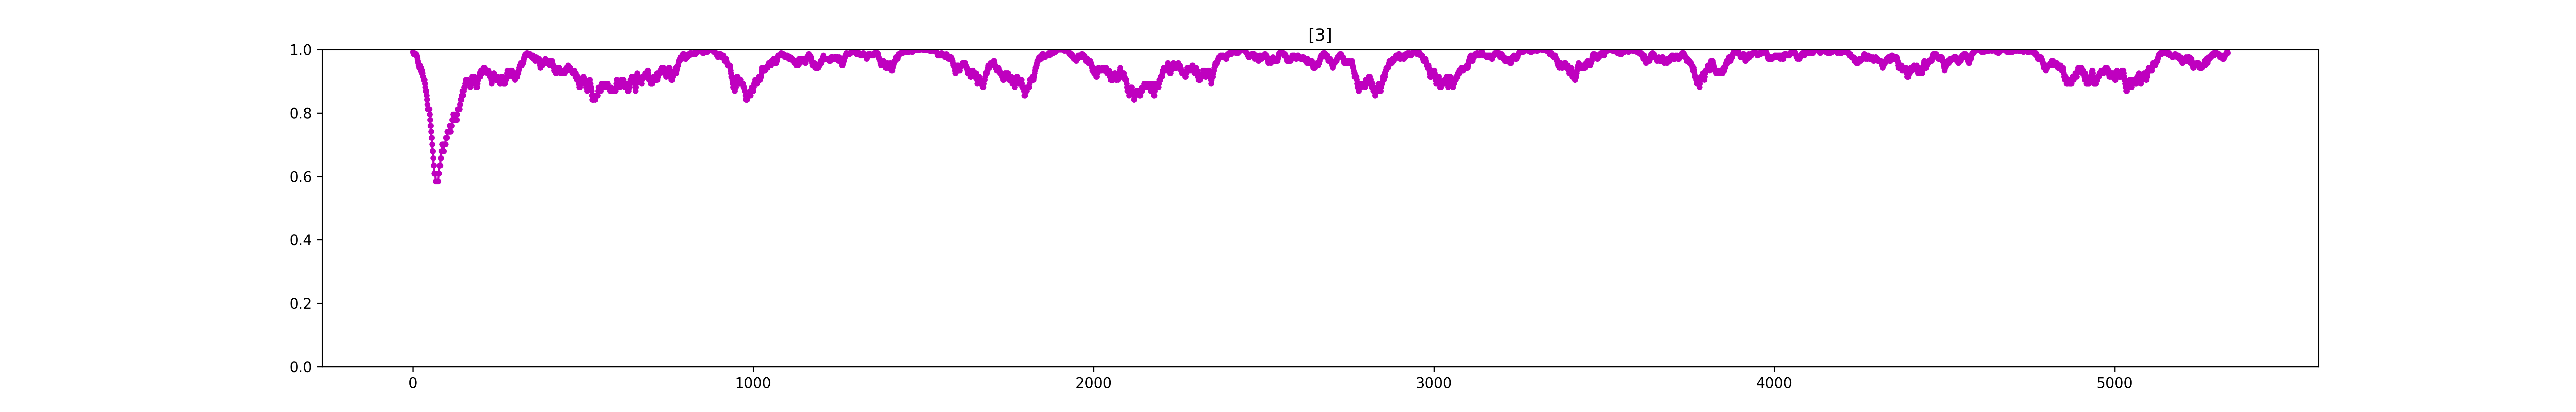
\includegraphics[scale=0.2]{src/main-matter/results/experiment-age/entropy/audio_aug/[3]/abc}
\caption{ABC podcast aaj-2019-04-26 untouched using SM[3]}

Ranked Probability: [(762, 'A'), (214, 'B')]
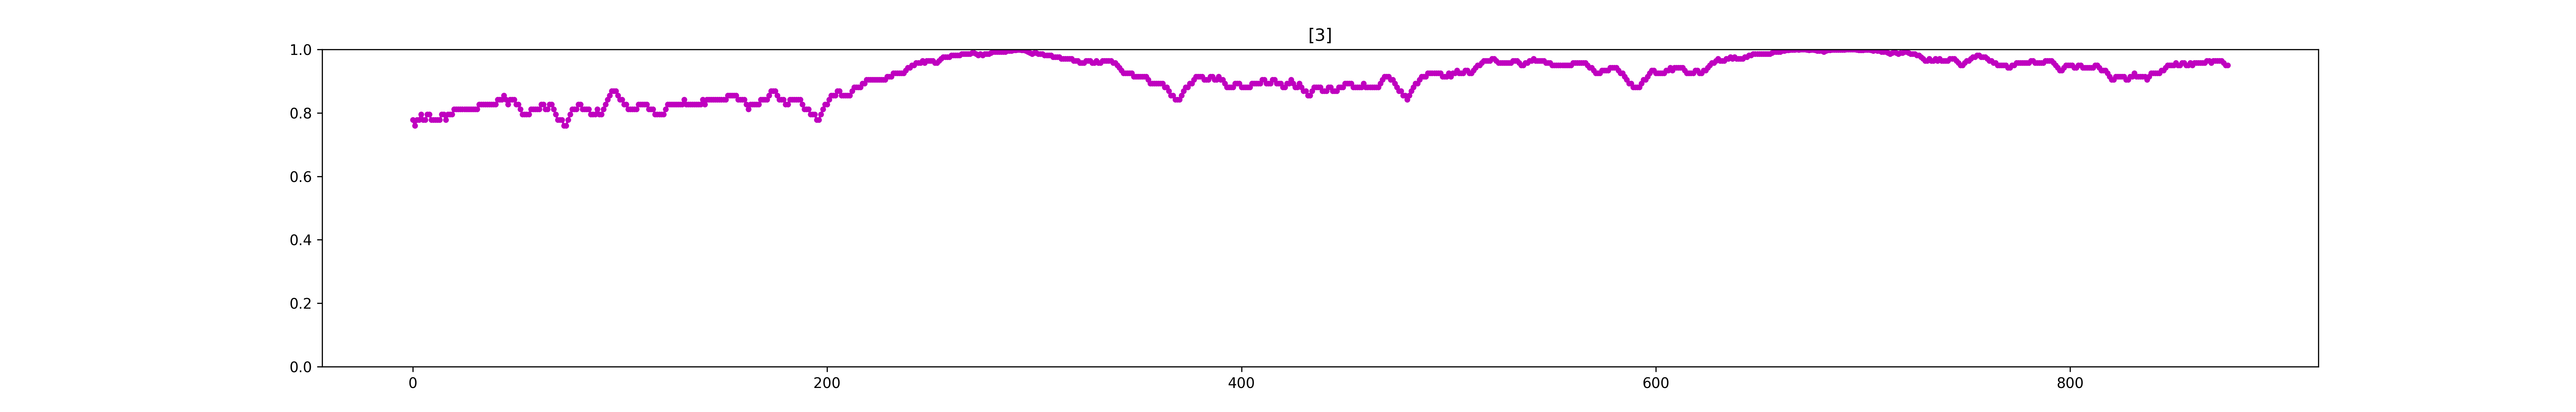
\includegraphics[scale=0.2]{src/main-matter/results/experiment-age/entropy/audio_aug/[3]/jjj}
\caption{JJJ podcast jmo-ali-barter untouched using SM[3]}

%\includegraphics[scale=0.2]{src/main-matter/results/experiment-age/entropy/audio_aug/[3]/abc-with-end-jjj}
%\caption{ABC podcast with JJJ inserted at the end using model [3]}

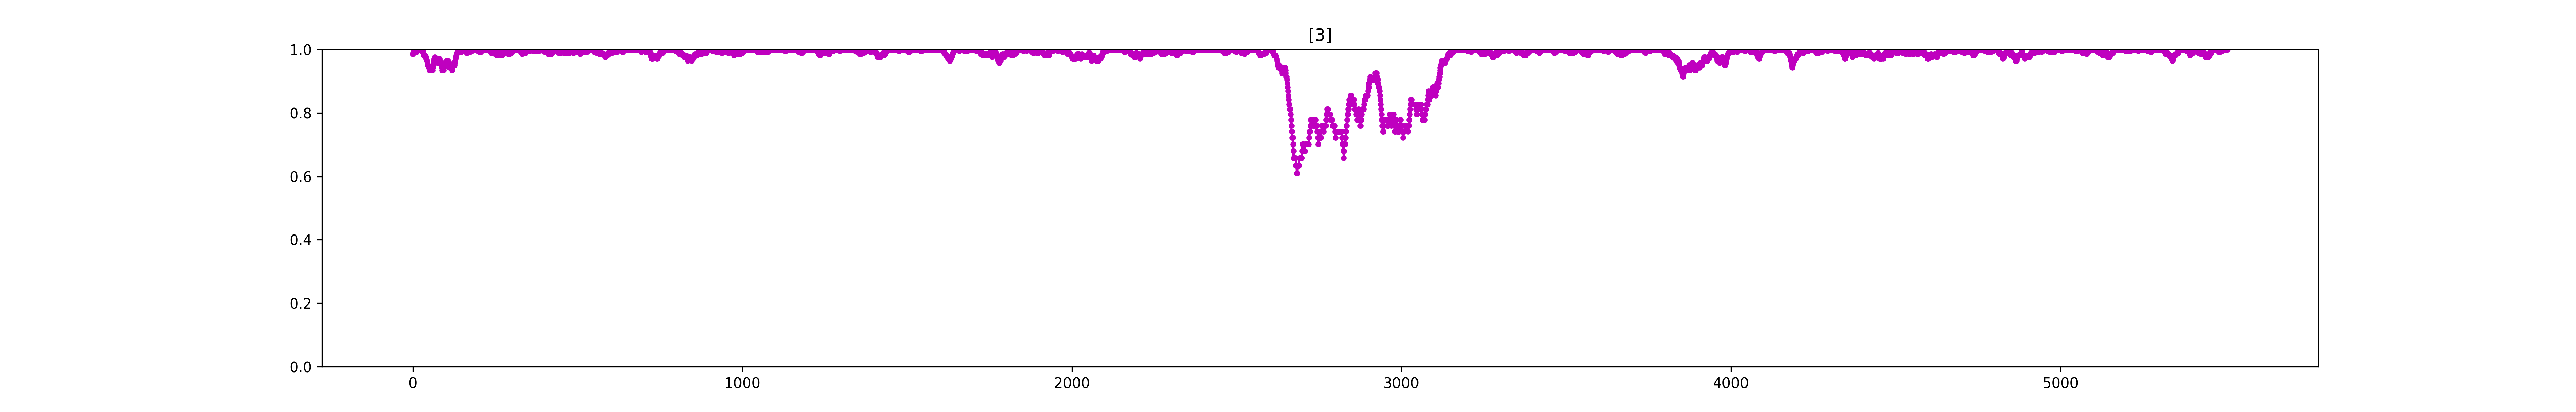
\includegraphics[scale=0.2]{src/main-matter/results/experiment-age/entropy/audio_aug/[3]/abc-middle-jjj}
\caption{ABC podcast with JJJ inserted in the middle using SM[3]}
%
%\includegraphics[scale=0.2]{src/main-matter/results/experiment-age/entropy/audio_aug/[3]/jjj-with-end-abc}
%\caption{JJJ podcast with ABC inserted at the end using model [3]}
%
%\includegraphics[scale=0.2]{src/main-matter/results/experiment-age/entropy/audio_aug/[3]/jjj-with-middle-abc}
%\caption{JJJ podcast with ABC inserted in the middle using model [3]}


\label{default}
\end{center}
\end{figure}




\clearpage

\subsubsection{Experiment 2.2.2 - Investigating Bin Width - SM[10]}
%This symbol model was produced using symbolisation approach SA1 (as shown in section x.x wtih fig x.x). 

%File 1: aaj-2019-04-26 \\
%Ranked Probability: [(5294, 'A'), (138, 'B')] \\
%
%File 2: jmo-2019-02-26-inspired-ali-barter---girlie-bits \\
% Ranked Probability: [(762, 'A'), (214, 'B')] \\
%
%Window Size: 100 \\
%Window Overlap: 99 \\
%Model: [10] \\

%\paragraph{Mean}
%Mean was --
%
%\paragraph{Range}
%Range was roughly the same for both \\
%
%\paragraph{Variance}
%ABC was much less consistent, varying between the range values constantly meaning frequent change in information delivery. \\

\begin{figure}[h]
\begin{center}

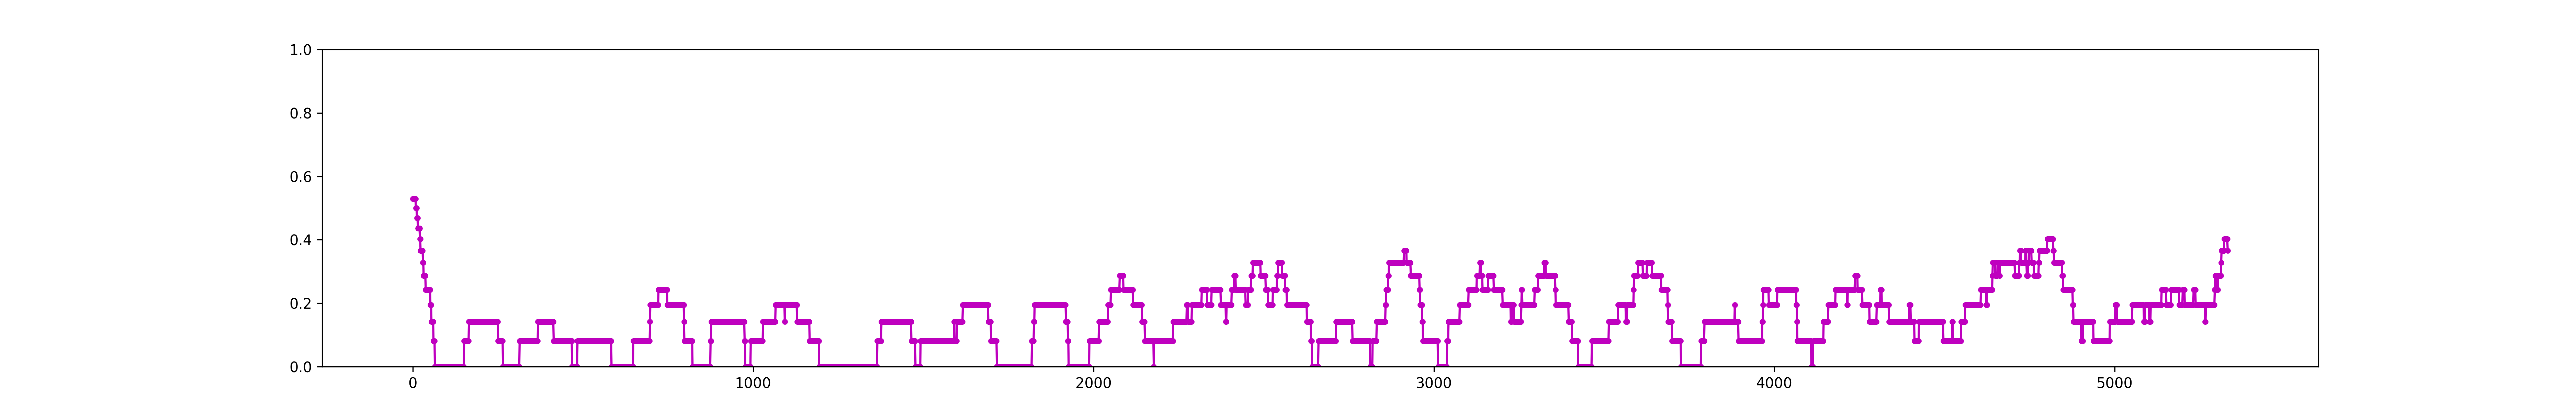
\includegraphics[scale=0.2]{src/main-matter/results/experiment-age/entropy/audio_aug/[10]/aaj-2019-04-26}
\caption{ABC podcast aaj-2019-04-26 untouched using model [10]}

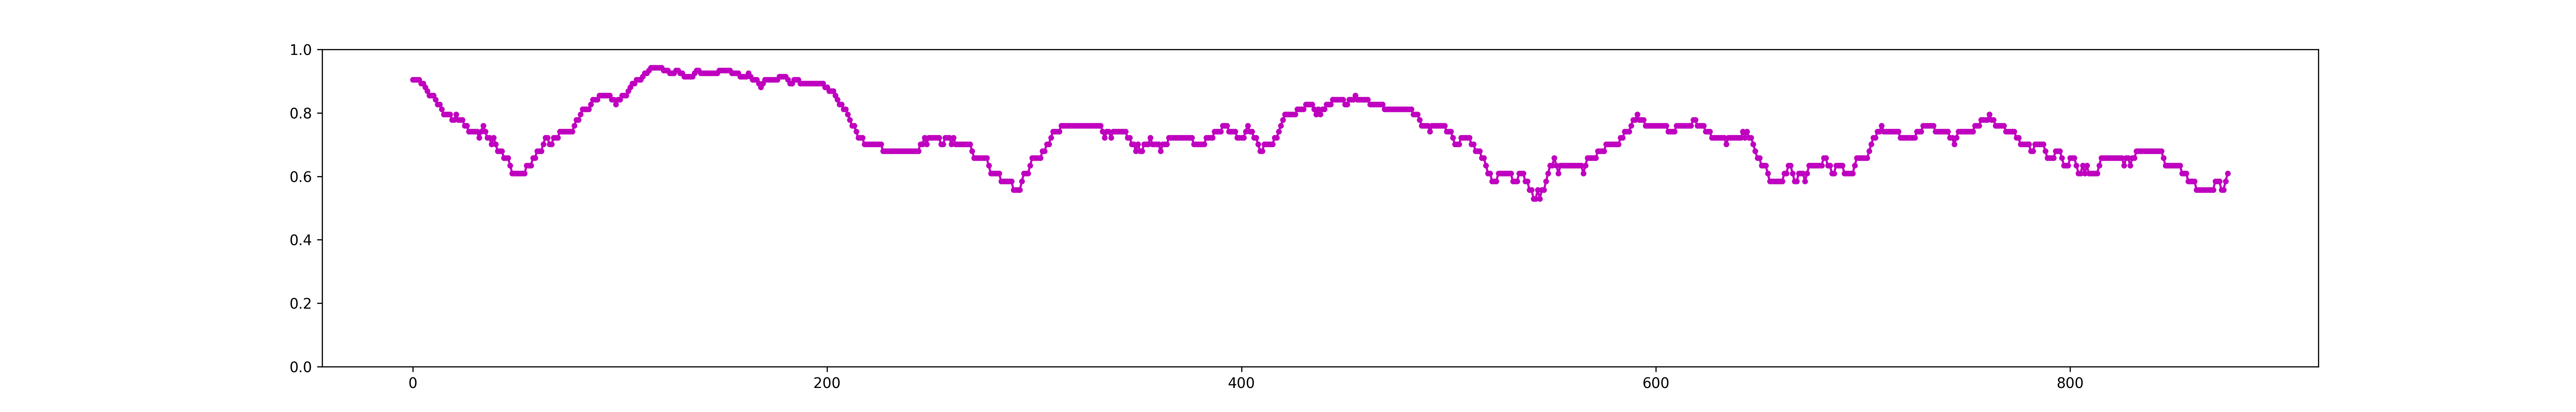
\includegraphics[scale=0.2]{src/main-matter/results/experiment-age/entropy/audio_aug/[10]/jmo-ali-barter}
\caption{JJJ podcast jmo-ali-barter untouched using model [10]}

%\includegraphics[scale=0.2]{src/main-matter/results/experiment-age/entropy/audio_aug/[10]/abc-with-end-jjj}
%\caption{ABC podcast with JJJ inserted at the end using model [10]}

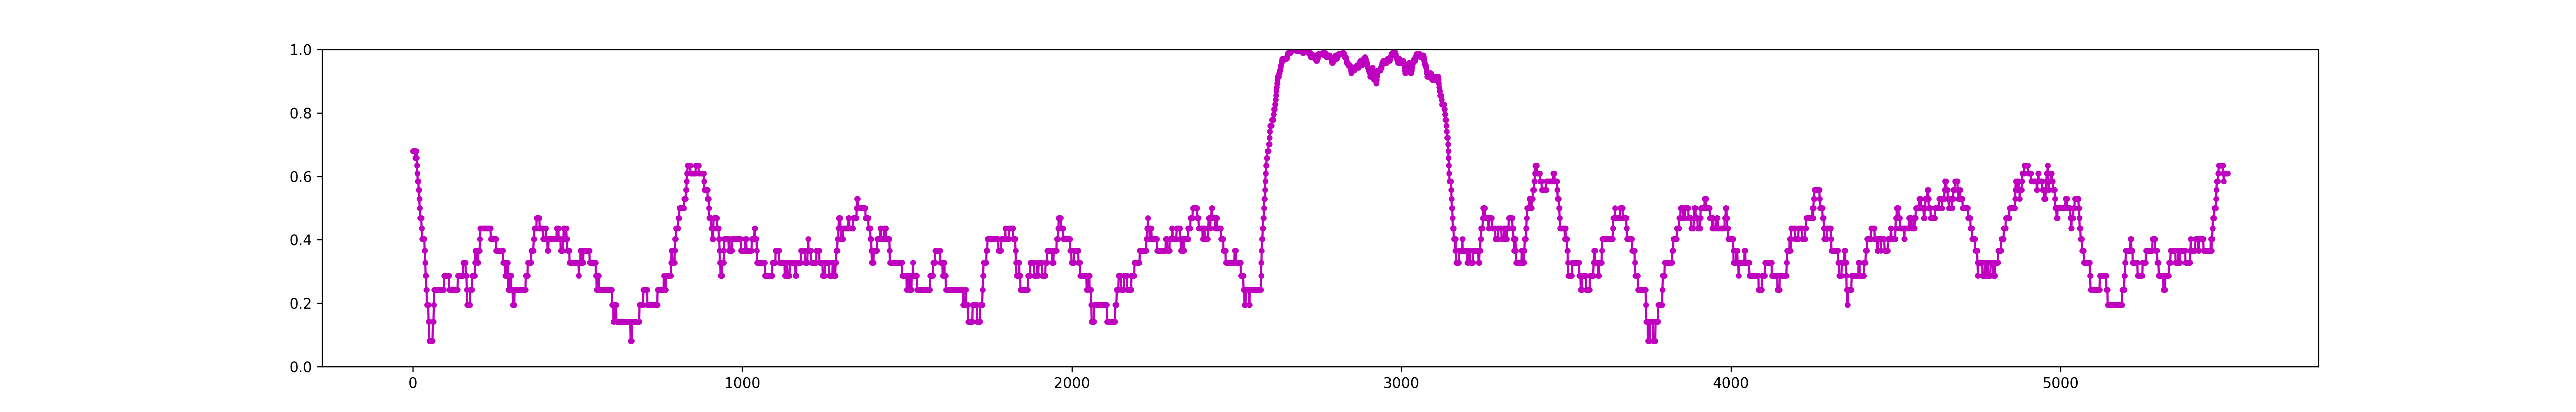
\includegraphics[scale=0.2]{src/main-matter/results/experiment-age/entropy/audio_aug/[10]/abc-with-middle-jjj}
\caption{ABC podcast with JJJ inserted in the middle using model [10]}

%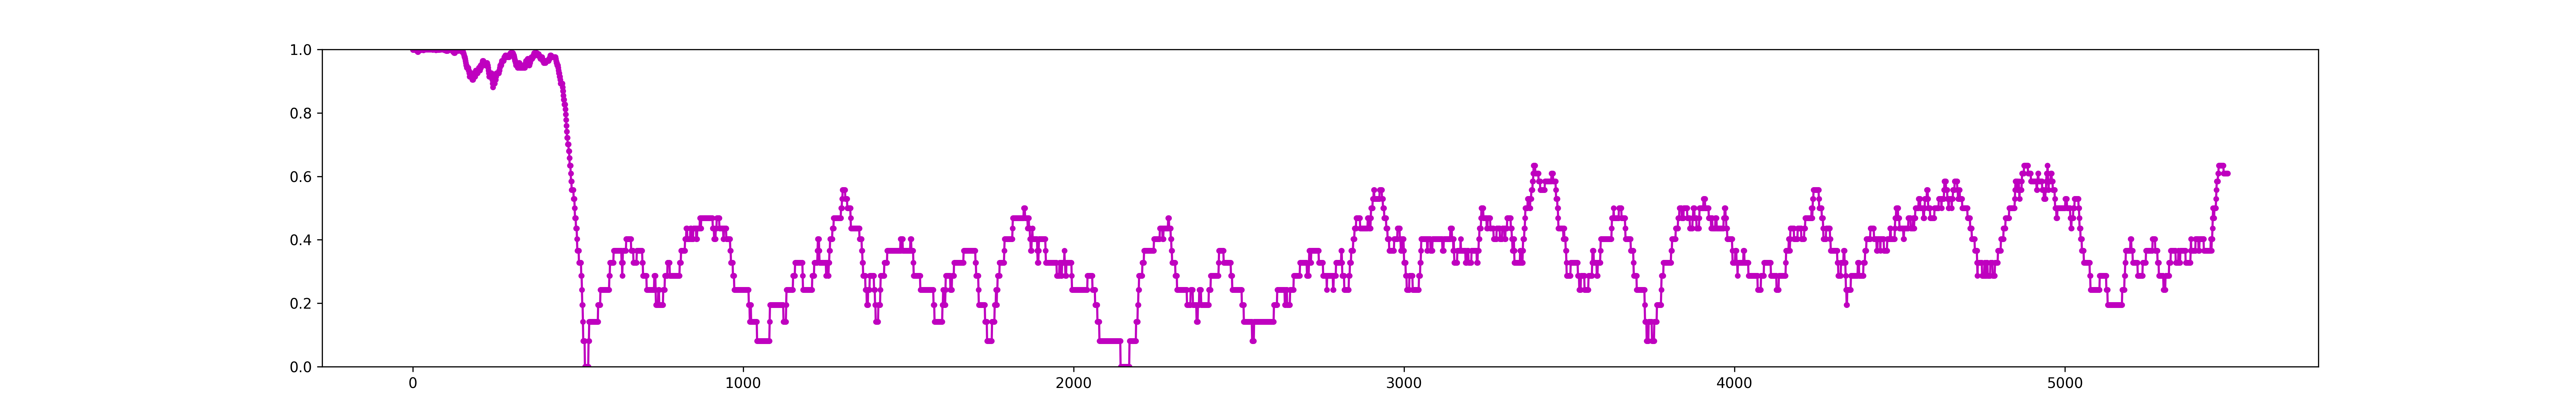
\includegraphics[scale=0.2]{src/main-matter/results/experiment-age/entropy/audio_aug/[10]/jjj-with-end-abc}
%\caption{JJJ podcast with ABC inserted at the end using model [10]}
%
%\includegraphics[scale=0.2]{src/main-matter/results/experiment-age/entropy/audio_aug/[10]/jjj-with-middle-abc}
%\caption{JJJ podcast with ABC inserted in the middle using model [10]}


\label{default}
\end{center}
\end{figure}


\subsubsection{Experiment 2.2.3 - Investigating Bin Width - SM[20]}

%Model: [20] \\

%\paragraph{Mean}
%Mean was --
%
%\paragraph{Range}
%Range was roughly the same for both \\
%
%\paragraph{Variance}
%ABC was much less consistent, varying between the range values constantly meaning frequent change in information delivery. \\


\begin{figure}[b!]
\begin{center}

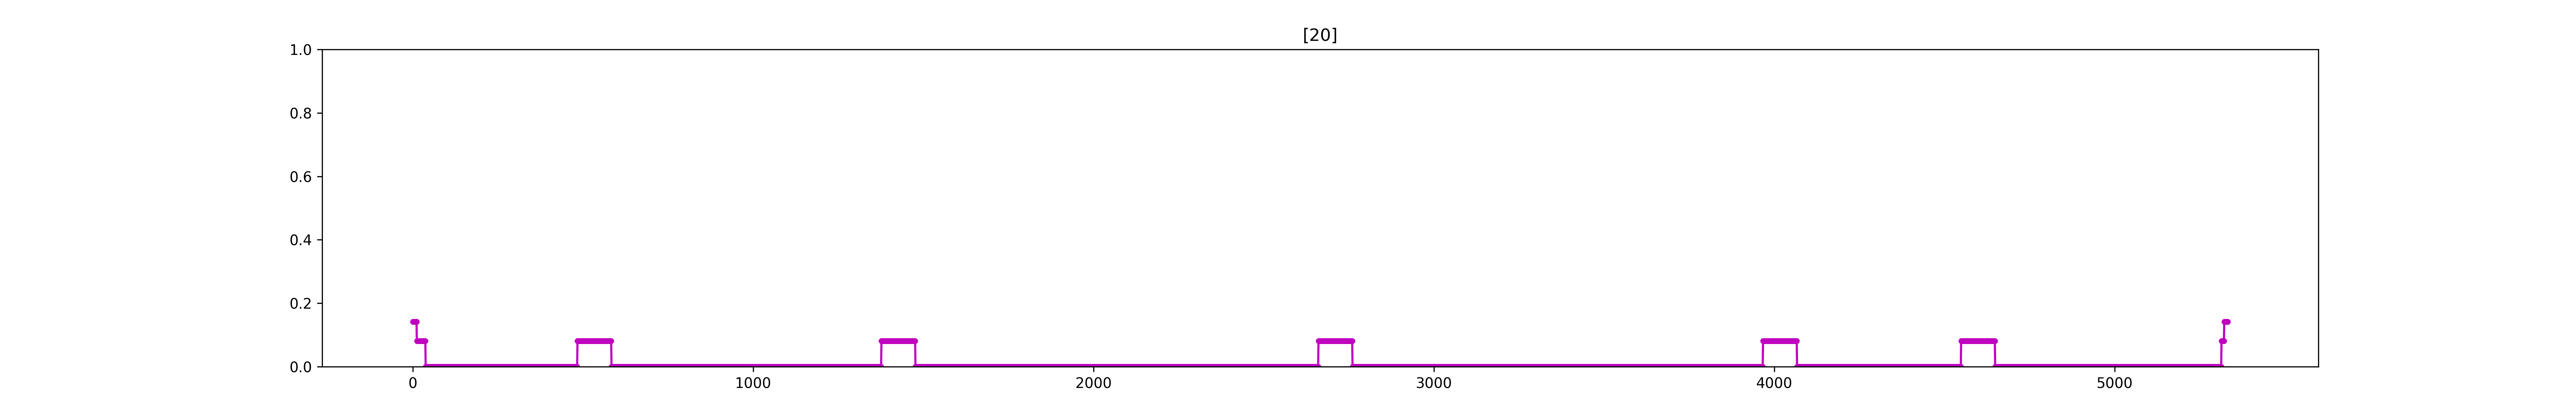
\includegraphics[scale=0.2]{src/main-matter/results/experiment-age/entropy/audio_aug/[20]/abc}
\caption{ABC podcast aaj-2019-04-26 untouched using model [20]}

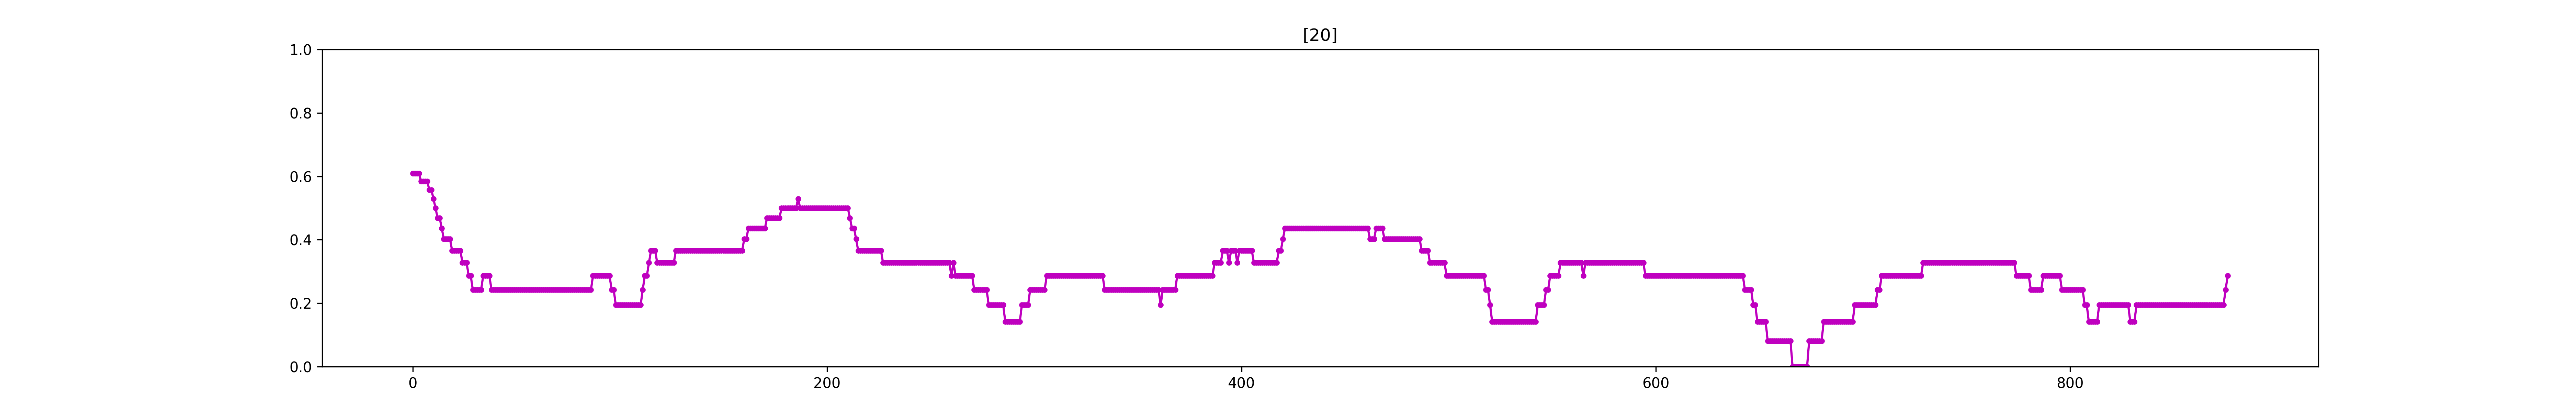
\includegraphics[scale=0.2]{src/main-matter/results/experiment-age/entropy/audio_aug/[20]/jjj}
\caption{JJJ podcast jmo-ali-barter untouched using model [20]}

%\includegraphics[scale=0.2]{src/main-matter/results/experiment-age/entropy/audio_aug/[10]/abc-with-end-jjj}
%\caption{ABC podcast with JJJ inserted at the end using model [10]}

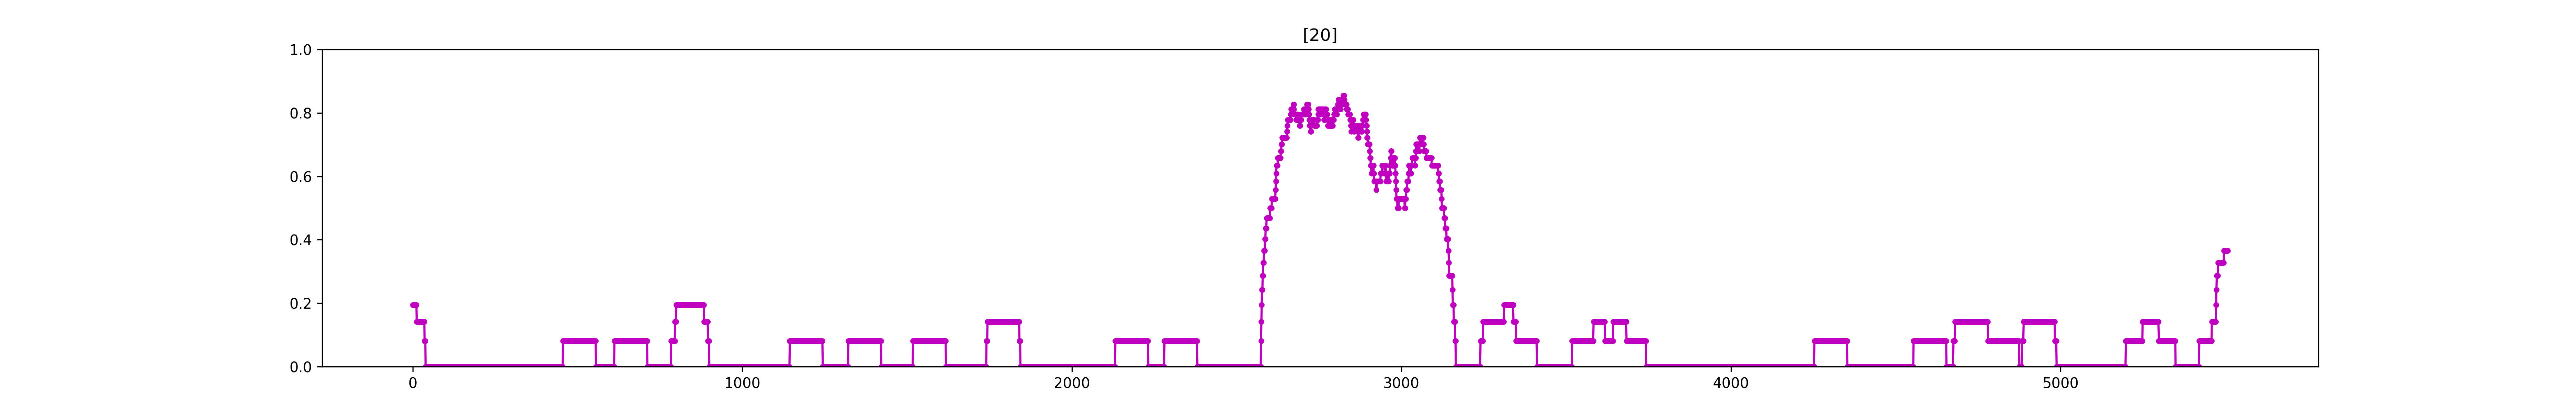
\includegraphics[scale=0.2]{src/main-matter/results/experiment-age/entropy/audio_aug/[20]/abc-middle-jjj}
\caption{ABC podcast with JJJ inserted in the middle using model [20]}

\label{default}
\end{center}
\end{figure}


%\clearpage


\newpage



\subsubsection{Experiment 2.2.4 - SA2 - SM[3,6,10,15]}
This symbol model was produced using Symbolisation Approach 2. 
%
%File 1: aaj-2019-04-26 \\
%Ranked Probability: [(3343, 'A'), (1360, 'B'), (591, 'C'), (111, 'D'), (27, 'E')] \\
%
%File 2: jmo-2019-02-26-inspired-ali-barter---girlie-bits \\
%Ranked Probability: [(330, 'A'), (266, 'B'), (166, 'C'), (114, 'D'), (100, 'E')] \\
%
%Window Size: 100 \\
%Window Overlap: 99 \\
%Model: [3,6,10,15] \\

%\paragraph{Mean}
%Mean was --
%
%\paragraph{Range}
%Range was roughly the same for both \\
%
%\paragraph{Variance}
%ABC was much less consistent, varying between the range values constantly meaning frequent change in information delivery. \\


\begin{figure}[htbp]
\begin{center}

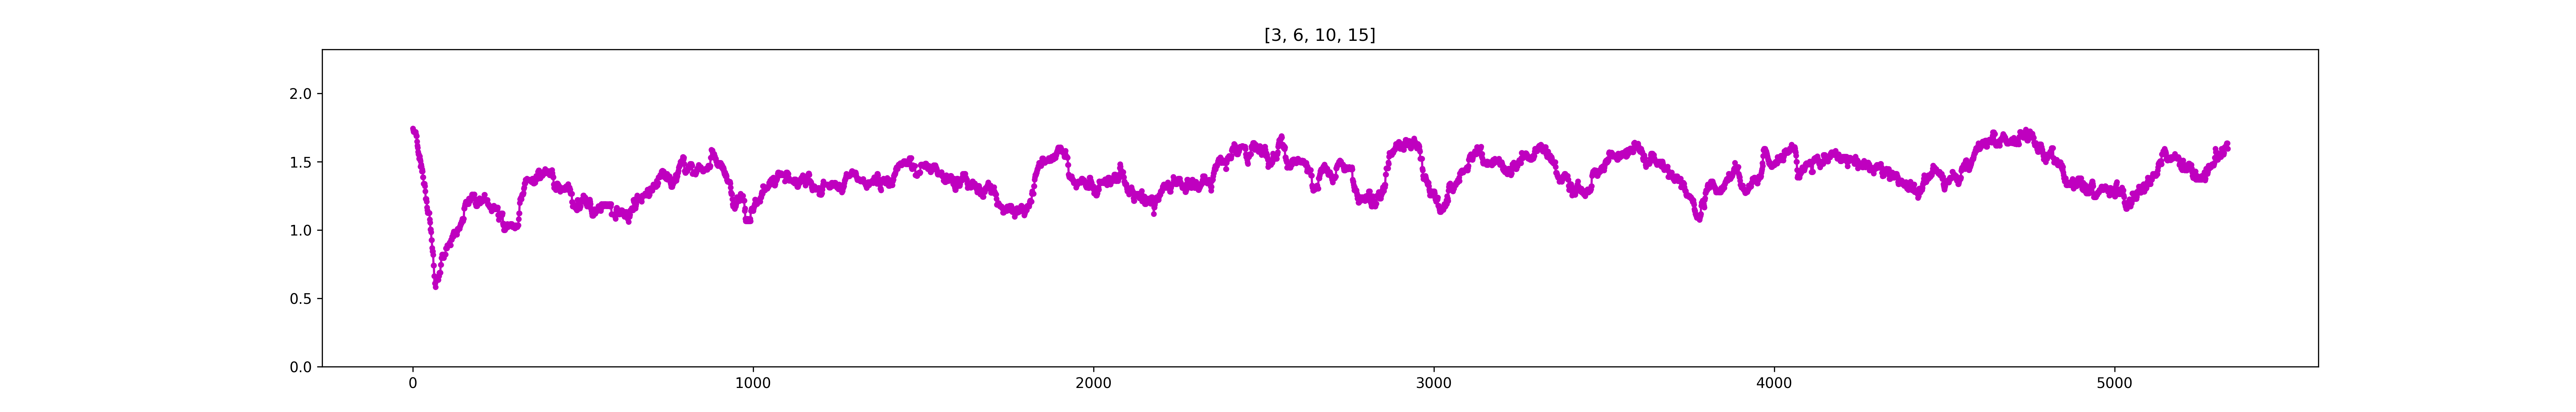
\includegraphics[scale=0.2]{src/main-matter/results/experiment-age/entropy/audio_aug/[3,6,10,15]/abc}
\caption{abc podcast aaj-2019-04-26 untouched model [3,6,10,15]}

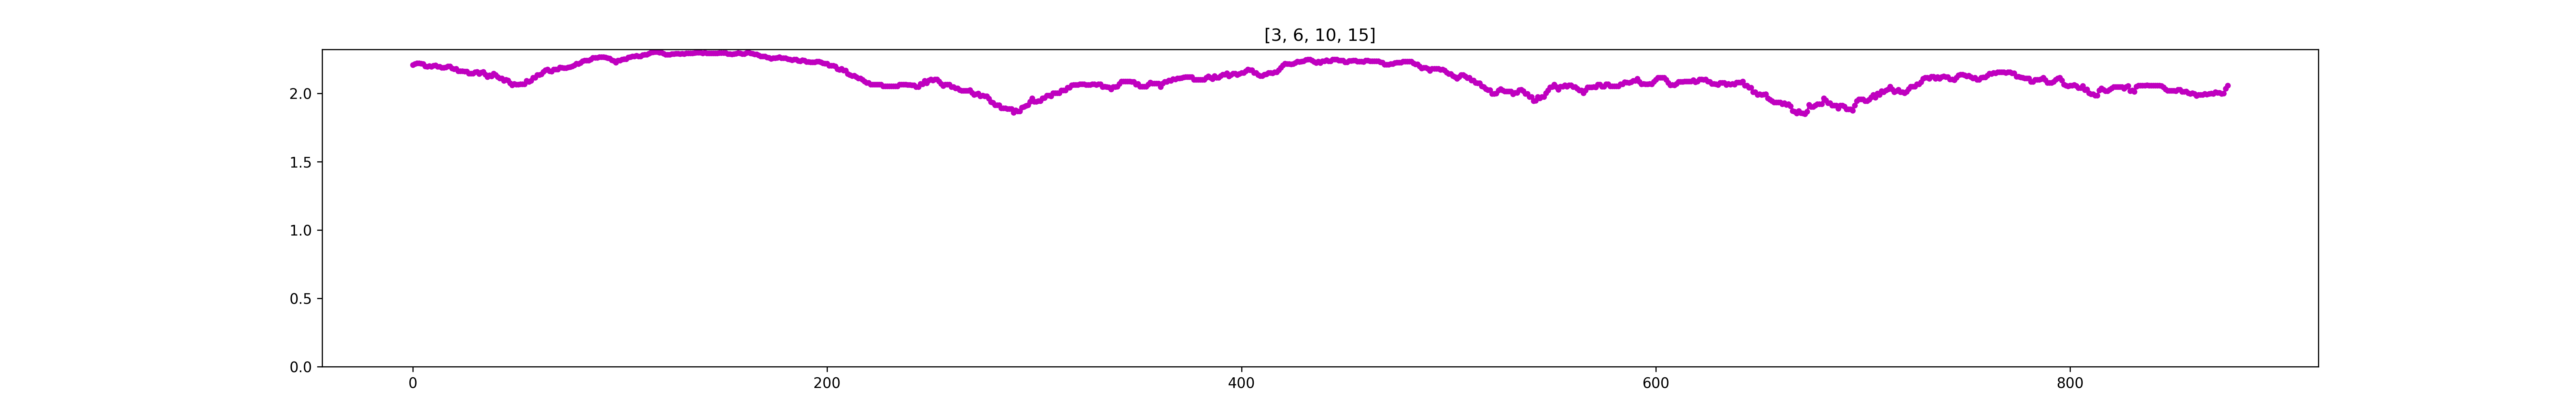
\includegraphics[scale=0.2]{src/main-matter/results/experiment-age/entropy/audio_aug/[3,6,10,15]/jjj}
\caption{jjj podcast jmo-ali-barter untouched model [3,6,10,15]}

%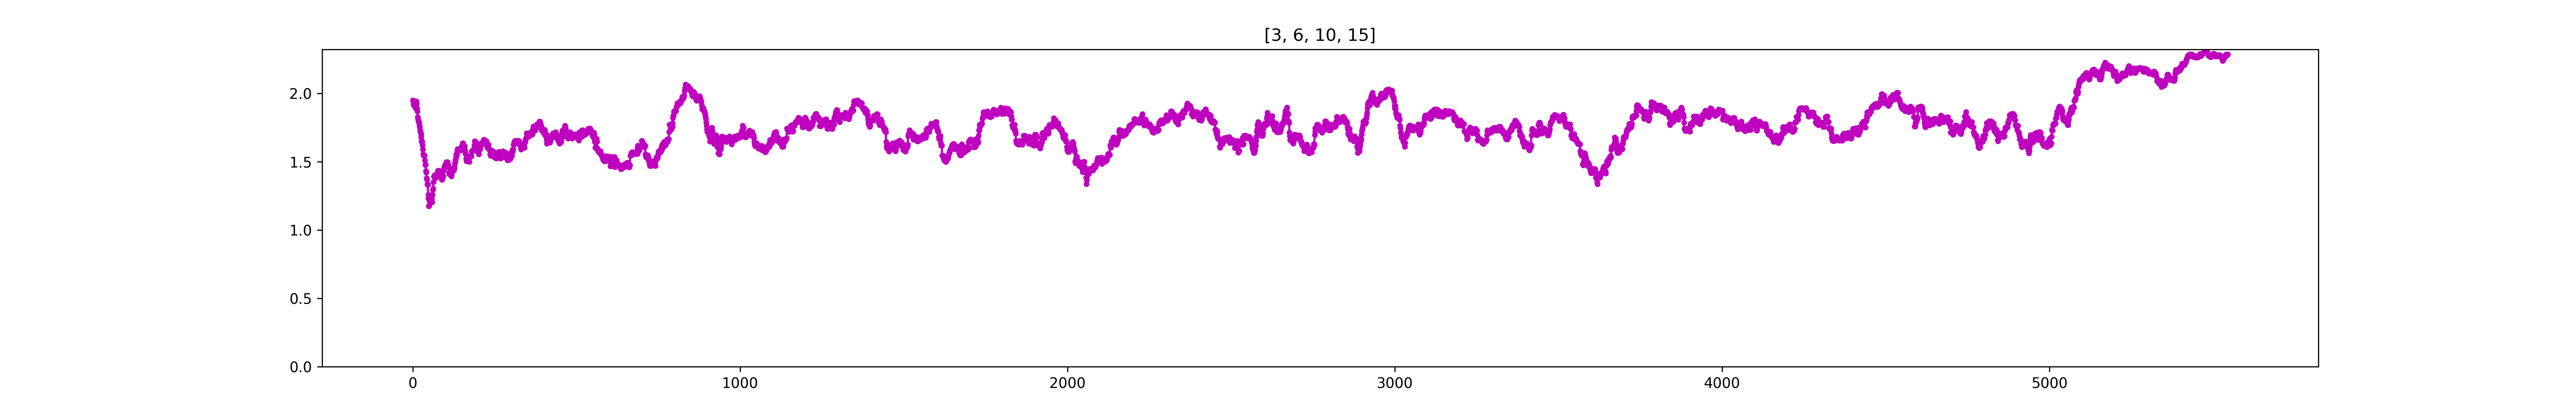
\includegraphics[scale=0.2]{src/main-matter/results/experiment-age/entropy/audio_aug/[3,6,10,15]/abc-with-end-jjj}
%\caption{abc podcast with jjj inserted at the end model [3,6,10,15]}

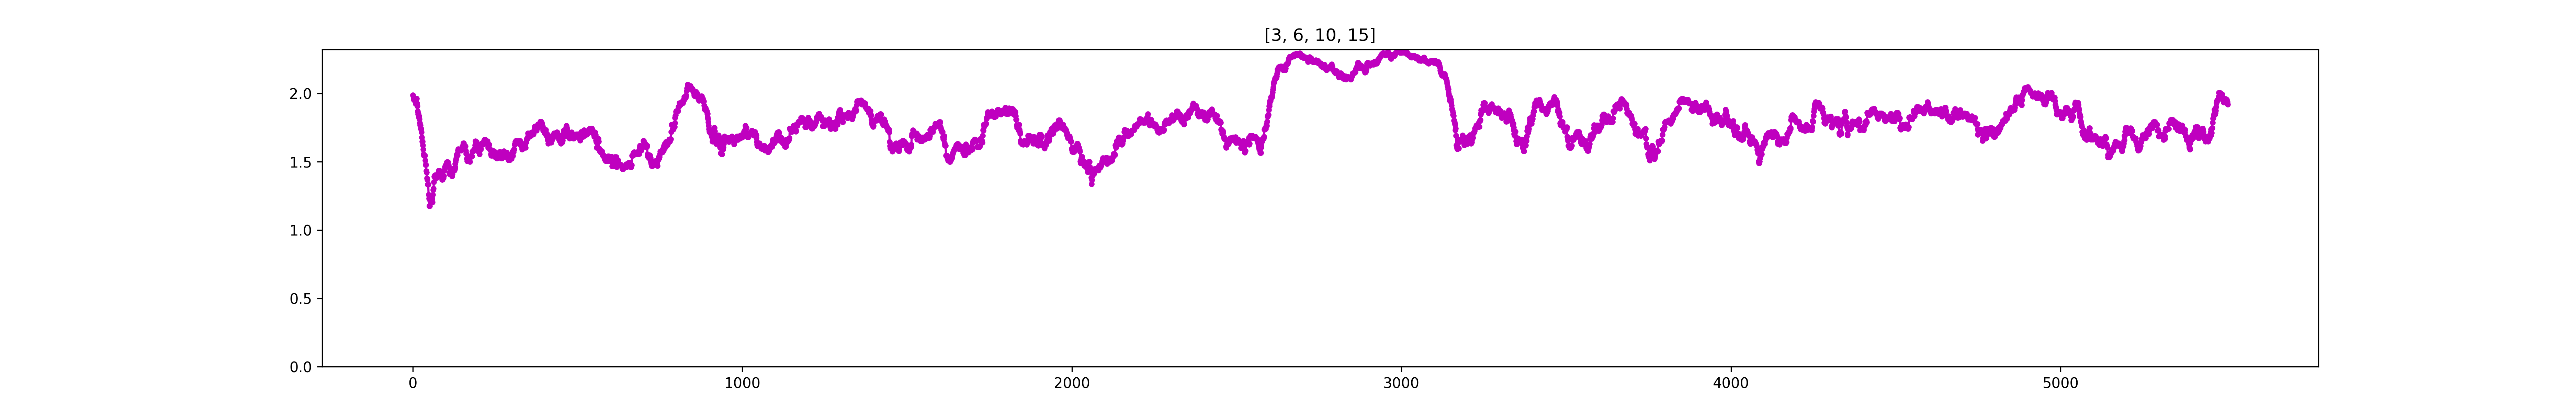
\includegraphics[scale=0.2]{src/main-matter/results/experiment-age/entropy/audio_aug/[3,6,10,15]/abc-middle-jjj}
\caption{abc podcast with jjj inserted in the middle model [3,6,10,15]}

%\includegraphics[scale=0.2]{src/main-matter/results/experiment-age/entropy/audio_aug/[3,6,10,15]/jjj-with-end-abc}
%\caption{jjj podcast with abc inserted at the end model [3,6,10,15]}
%
%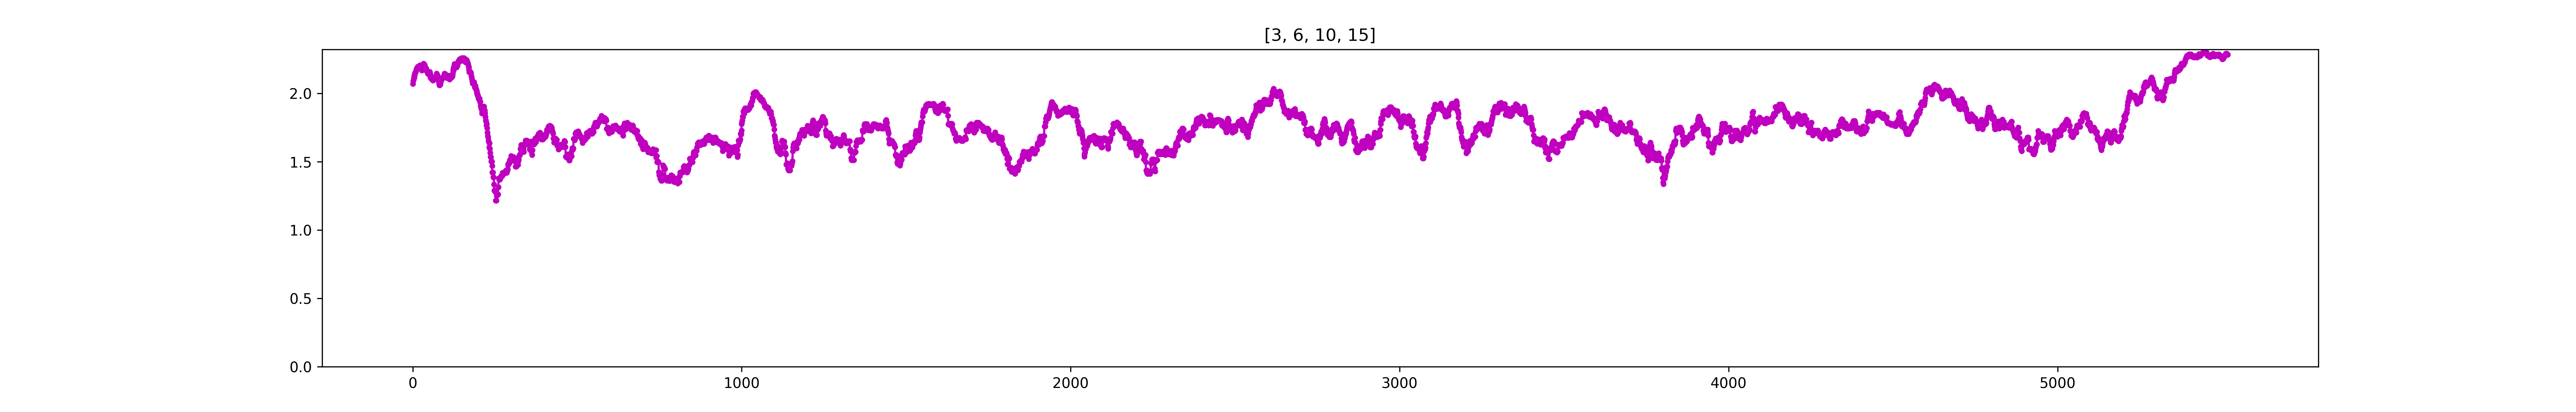
\includegraphics[scale=0.2]{src/main-matter/results/experiment-age/entropy/audio_aug/[3,6,10,15]/jjj-with-middle-abc}
%\caption{jjj podcast with abc inserted in the middle model [3,6,10,15]}


\label{default}
\end{center}
\end{figure}


%\clearpage
\pagebreak



\subsection{Experiment 2.3 - Investigating Audio Splice Position}

\begin{figure}[b!]
\begin{center}

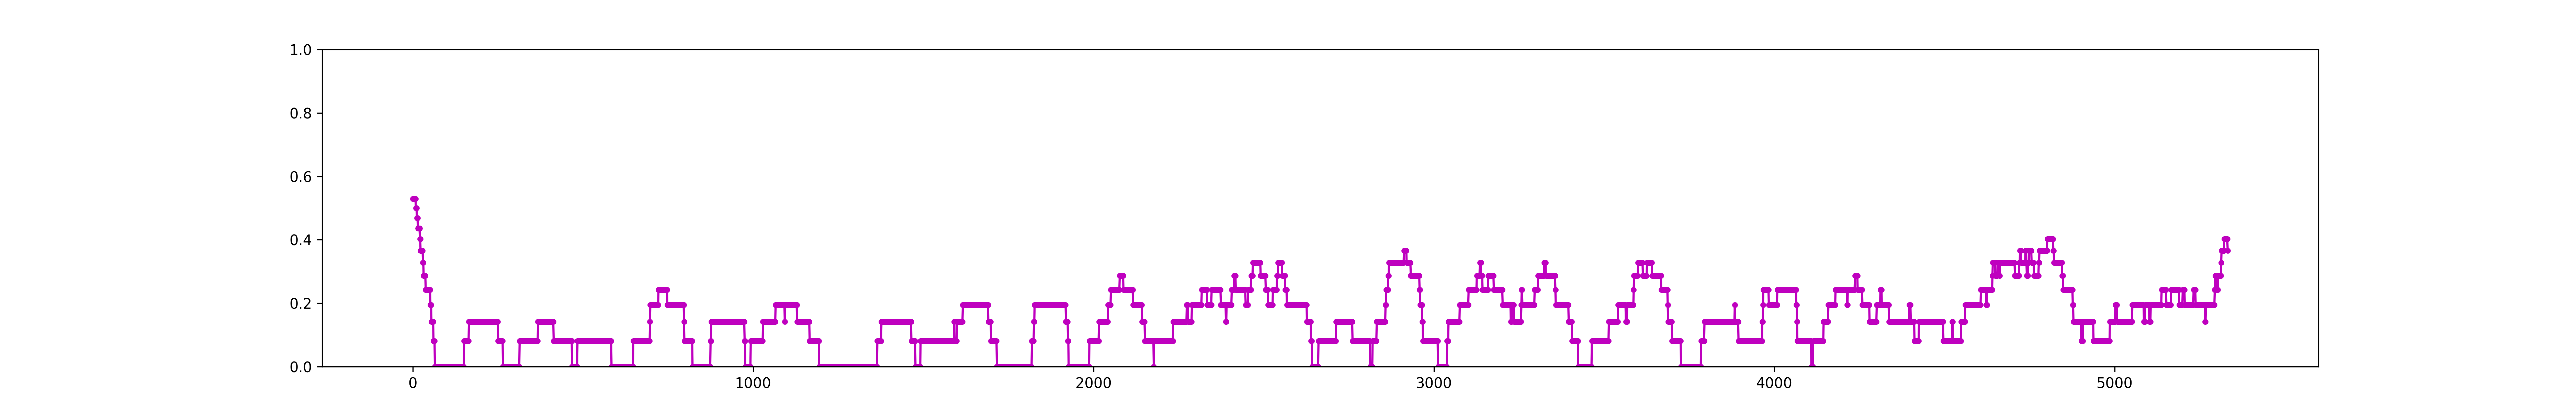
\includegraphics[scale=0.2]{src/main-matter/results/experiment-age/entropy/audio_aug/[10]/aaj-2019-04-26}
\caption{ABC podcast aaj-2019-04-26 untouched using model [10]}

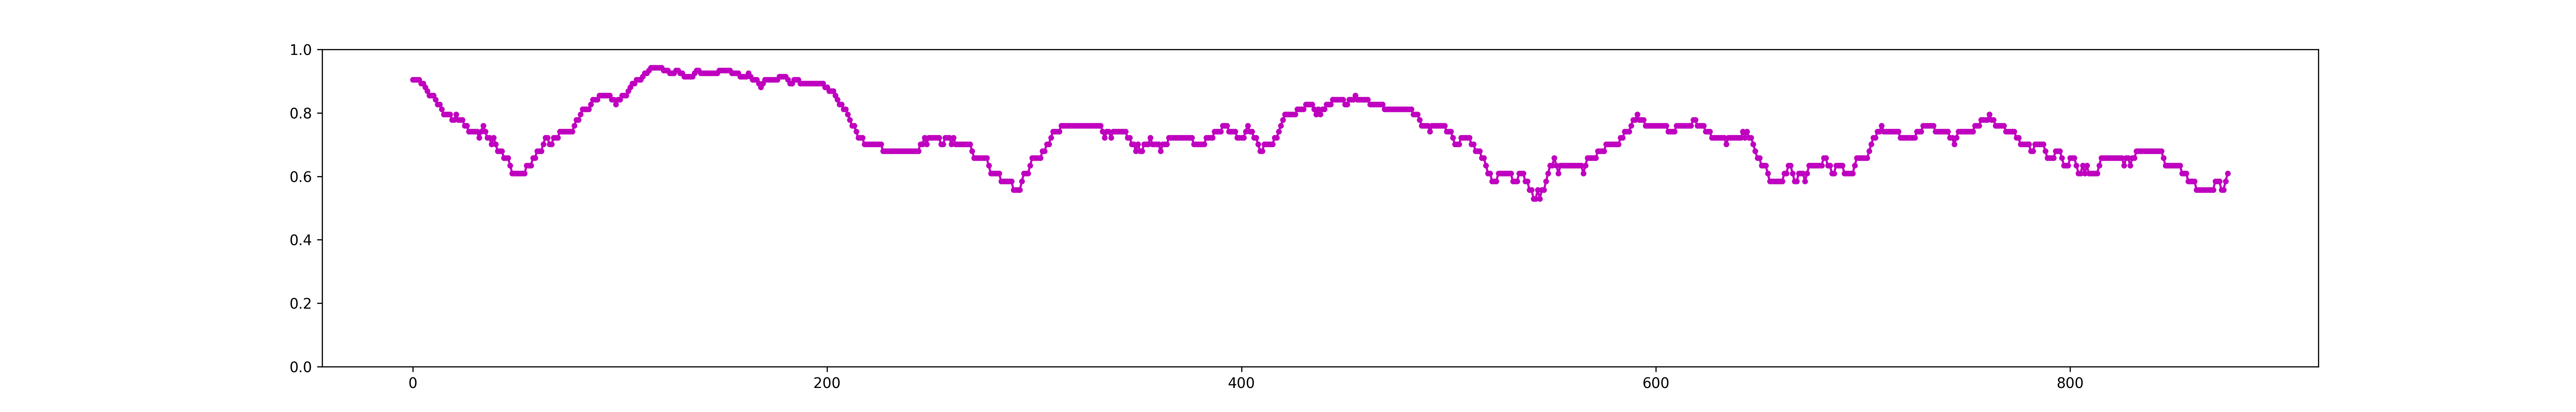
\includegraphics[scale=0.2]{src/main-matter/results/experiment-age/entropy/audio_aug/[10]/jmo-ali-barter}
\caption{JJJ podcast jmo-ali-barter untouched using model [10]}

\includegraphics[scale=0.2]{src/main-matter/results/experiment-age/entropy/audio_aug/[10]/abc-with-end-jjj}
\caption{ABC podcast with JJJ inserted at the end using model [10]}

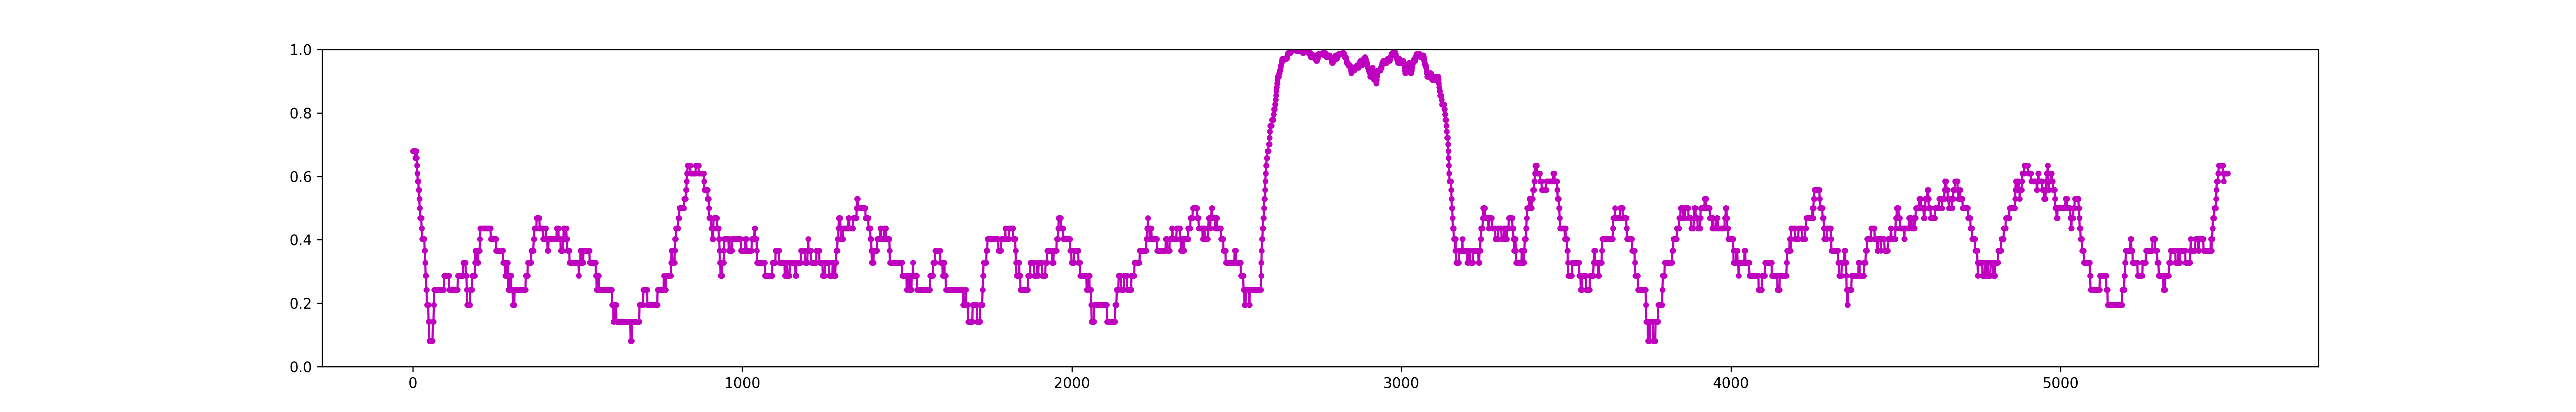
\includegraphics[scale=0.2]{src/main-matter/results/experiment-age/entropy/audio_aug/[10]/abc-with-middle-jjj}
\caption{ABC podcast with JJJ inserted in the middle using model [10]}

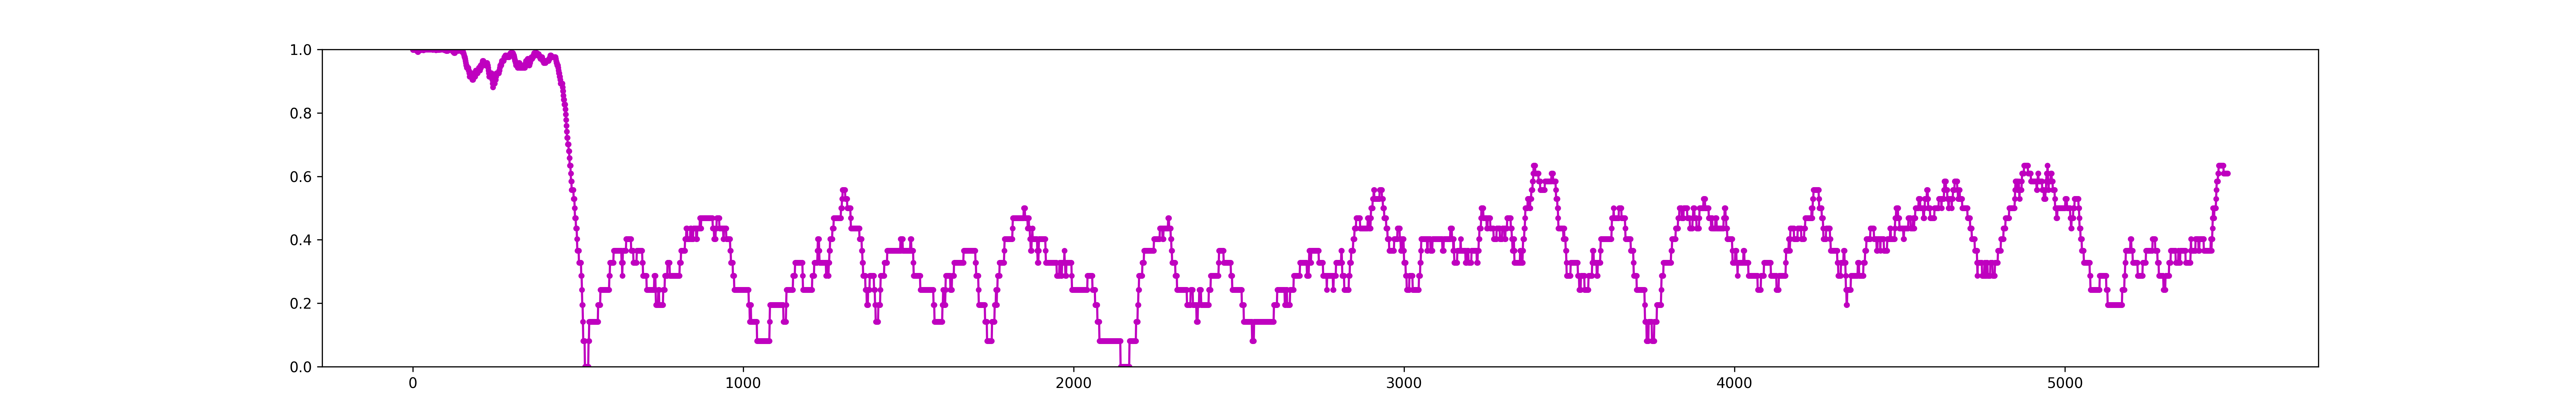
\includegraphics[scale=0.2]{src/main-matter/results/experiment-age/entropy/audio_aug/[10]/jjj-with-end-abc}
\caption{JJJ podcast with ABC inserted at the end using model [10]}

\includegraphics[scale=0.2]{src/main-matter/results/experiment-age/entropy/audio_aug/[10]/jjj-with-middle-abc}
\caption{JJJ podcast with ABC inserted in the middle using model [10]}


\label{default}
\end{center}
\end{figure}


\clearpage
